\documentclass[12pt,a4paper]{article}
\usepackage[T1]{fontenc}
\usepackage{lmodern}
\usepackage{amsmath,amssymb,amsthm}
\usepackage{graphicx}
\usepackage[margin=2.0cm]{geometry} 
\usepackage{setspace}    
\setstretch{1.1}
\usepackage{enumitem}
\usepackage{hyperref} % se puede añadir hidelinks para evitar cuadros alrededor de los enlaces
\usepackage[all]{hypcap} % jump to top of figure, not caption
\usepackage{url}
\usepackage{fontawesome5}
\usepackage{tikz}
\usepackage{tikz-cd}
\usepackage{tikz-3dplot}
\usetikzlibrary{angles,quotes,arrows.meta,calc,babel,3d,positioning}
\usepackage{lipsum}
\usepackage{listings}
\usepackage{fancyhdr}
\usepackage{xcolor} % Added for colors
\usepackage{titlesec} % Added for title formatting
\usepackage{array}
\usepackage{booktabs}
\usepackage{float}
\usepackage{wrapfig} % For text wrapping around figures
\usepackage{microtype}
\usepackage[ngerman]{babel}
\usepackage{csquotes}
\usepackage[backend=biber,style=ieee,sorting=nyt,backref=true]{biblatex}
\DeclareAutoCiteCommand{footfull}{\footfullcite}{\footfullcites}
\ExecuteBibliographyOptions{autocite=footfull}

% Shorten footnote citations to crucial info


\AtEveryCitekey{%
  \clearfield{url}%
  \clearfield{urldate}%
  \clearfield{doi}%
  \clearfield{issn}%
  \clearfield{isbn}%
  \clearfield{note}%
  \clearfield{volume}%
  \clearfield{number}%
  \clearfield{pages}%
  \clearfield{journaltitle}%
  \clearfield{booktitle}%
  \clearfield{eventtitle}%
  \clearfield{howpublished}%
  \clearlist{publisher}%
  \clearlist{location}%
  \clearname{editor}%
  \iffieldundef{shorttitle}{}{\clearfield{title}\clearfield{subtitle}}%
}

% Make sure shorttitle is printed if title is cleared
\renewbibmacro*{title}{%
  \iffieldundef{title}
    {\iffieldundef{shorttitle}
       {}
       {\printfield[title]{shorttitle}}}
    {\printfield[title]{title}}%
}

\addbibresource{references.bib}

% Better figure placement defaults
\setcounter{topnumber}{2}
\setcounter{bottomnumber}{2}
\setcounter{totalnumber}{4}
\renewcommand{\topfraction}{0.85}
\renewcommand{\bottomfraction}{0.85}
\renewcommand{\textfraction}{0.15}
\renewcommand{\floatpagefraction}{0.7}

% Define colors
\definecolor{titlecolor}{RGB}{0, 51, 102}
\definecolor{codebg}{RGB}{245, 245, 245}
\definecolor{codecomment}{RGB}{92, 99, 112}
\definecolor{codekeyword}{RGB}{30, 64, 175}
\definecolor{codestring}{RGB}{14, 116, 144}

% Month-year without day
\newcommand{\monthyear}{%
    \ifcase\month\or Januar\or Februar\or M\"arz\or April\or Mai\or Juni\or Juli\or August\or September\or Oktober\or November\or Dezember\fi\space \number\year
}

\lstdefinestyle{code}{
    language=bash,
    basicstyle=\ttfamily\small,
    keywordstyle=\color{codekeyword},
    commentstyle=\color{codecomment},
    stringstyle=\color{codestring},
    backgroundcolor=\color{codebg},
    showstringspaces=false,
    inputencoding=utf8,
    breaklines=true,
    frame=single,
    framerule=0.4pt,
    rulecolor=\color{black!20},
    xleftmargin=0.4em,
    xrightmargin=0.4em,
    aboveskip=0.8em,
    belowskip=0.8em,
    literate={ä}{{\"a}}1 {ö}{{\"o}}1 {ü}{{\"u}}1 {Ä}{{\"A}}1 {Ö}{{\"O}}1 {Ü}{{\"U}}1 {ß}{{\ss}}1 {–}{{--}}1
}
\lstset{style=code}

% Fix headheight warning
\setlength{\headheight}{14.5pt}
\addtolength{\topmargin}{-2.5pt}

% Consistent theorem/proof environments
\newtheorem{theorem}{Theorem}
\newtheorem{lemma}[theorem]{Lemma}
\newtheorem{corollary}[theorem]{Corollary}
\theoremstyle{definition}
\newtheorem{definition}[theorem]{Definition}
\newtheorem{problem}{Problem}

% Set up headers
\pagestyle{fancy}
\fancyhf{} % Clear all header and footer fields
\fancyhead[L]{Victor Gurbani}
\fancyhead[R]{JuFo 2026}
\fancyfoot[C]{\thepage} % Page number in center of footer

% Define a separate first page style with no numbers
\fancypagestyle{firstpage}{
    \fancyhf{} % Clear all header and footer fields
    \renewcommand{\headrulewidth}{0pt} % Remove header rule
    \renewcommand{\footrulewidth}{0pt} % Remove footer rule
}

% Create a custom title command
\renewcommand{\maketitle}{
    \begin{titlepage}
        \centering
        \vspace*{1cm}
        {\color{titlecolor}\rule{\linewidth}{1pt}}
        \vspace{1.5cm}

        {\fontsize{28}{34}\selectfont\color{titlecolor}\textbf{Empirische Musikalische Kartographie} \par Eine quantitative Modellierung der stilistischen Evolutionsdynamik von Bach bis Debussy\par}

        \vspace{1.5cm}
        {\color{titlecolor}\rule{\linewidth}{1pt}}
        \vspace{2cm}
        
        {\Large\textbf{Victor Gurbani}\par}
        \vspace{0.5cm}
        {\large \monthyear\par}
        
        \vfill
        % Optional: Add a simple decorative element
        % \begin{tikzpicture}[remember picture, overlay]
        %     \draw[color=titlecolor, line width=0.5pt] 
        %         ($(current page.center) + (-3,0)$) -- ($(current page.center) + (3,0)$);
        % \end{tikzpicture}
    \end{titlepage}
}
\newcommand{\linkurl}[1]{\href{#1}{\textcolor{blue}{\underline{\small\nolinkurl{#1}}}}}


\begin{document}

\maketitle
\hypersetup{pageanchor=false}
\pagenumbering{roman}
\newpage

    \tableofcontents

\newpage
\setcounter{page}{1}
\pagenumbering{arabic}
\hypersetup{pageanchor=true}

\section{Fachliche Kurzfassung}
Die vorliegende Arbeit untersucht die stilistische Entwicklung der Klaviermusik von Johann Sebastian Bach bis Claude Debussy durch einen quantitativen, dynamischen Ansatz. Anstatt Komponisten lediglich statisch zu klassifizieren, modelliert dieses Projekt die \enquote{Evolutionsgeschwindigkeit} musikalischer Merkmale über drei Jahrhunderte. Datengrundlage bilden 144 Solowerke (je 36 pro Komponist), aus denen mittels computergestützter Methoden 36 interpretierbare musikalische Features extrahiert wurden. Die statistische Auswertung bestätigt für 29 dieser Merkmale hochsignifikante epochenspezifische Veränderungen (FDR $q<0{,}05$), während eine Hauptkomponentenanalyse (PCA) belegt, dass 48,2\,\% der stilistischen Varianz durch die ersten drei Dimensionen erklärt werden.

Durch die Einführung von \enquote{Evolutionskoeffizienten} und die Anwendung eines \enquote{Difference-in-Differences}-Ansatzes (DDD) weisen wir nach, dass die Romantik eine dramatische Beschleunigung des Stilwandels darstellt. Insbesondere die Expansion des Ambitus (+25,14 Halbtöne DD-Wert) und die Zunahme der Dissonanz (+0,31 DD-Wert) markieren diesen evolutionären Sprung, während die rhythmische Komplexität erst bei Debussy signifikant ansteigt (+1,41 DD-Wert). Die PCA-Projektion visualisiert diese Befunde als dreidimensionale Landkarte: Chopin positioniert sich mathematisch nachweisbar als \enquote{Brückenfigur} zwischen klassischer Ordnung und impressionistischer Auflösung.

Alle Skripte, Daten und Visualisierungen sind dokumentiert und ermöglichen reproduzierbare Folgeuntersuchungen zur stilistischen Evolution in der westlichen Kunstmusik. Die vollständige Merkmalsdokumentation und Reproduzierbarkeitsanleitungen finden sich in \hyperref[app:A]{Anhang~\ref*{app:A}} und~\hyperref[app:B]{\ref*{app:B}}.

\section{Motivation und Fragestellung}
In der historischen Musikwissenschaft wird der Wandel von Epochen meist durch qualitative Stilmerkmale beschrieben. Die Frage, mit welcher Dynamik und in welche Richtung sich musikalische Parameter über die Zeit verändern, bleibt jedoch oft rein deskriptiv. Diese Arbeit verfolgt das Ziel, die Evolution der Musiksprache von der Barockzeit bis zum Impressionismus als messbare Trajektorie in einem multidimensionalen Merkmalsraum zu kartographieren.

Während bisherige Studien meist auf die Trennung von Stilen fokussierten\autocite[Vgl.][]{LinJeng1987, Simonetta2025}, rückt hier die \enquote{Vektorgeschwindigkeit} des Wandels in den Fokus. Lin-Jengs Pionierarbeit von 1987 versuchte bereits, Mozart, Chopin und Debussy mittels Prolog-Regeln zu unterscheiden, war jedoch durch manuelles DARMS-Encoding und kleine Stichproben limitiert. Moderne Ressourcen -- das 2024 veröffentlichte PDMX-MusikXML-Archiv\autocite{PDMX2024} mit 254\,077 Partituren und die \texttt{music21}-Bibliothek\autocite{Cuthbert2010} -- ermöglichen nun eine skalierbare Neubearbeitung.

Besonders Chopin nimmt dabei eine Schlüsselrolle ein: Er wird hier mathematisch als \enquote{Brückenfigur} verifiziert, an der die stilistische Beschleunigung der Romantik messbar kulminiert. Unter Verwendung des \textit{music21}-Frameworks soll die traditionelle Analyse durch eine empirische Kartographie ergänzt werden, die den \enquote{Puls} der Musikgeschichte greifbar macht.

\subsection{Forschungsfragen}
Daraus ergeben sich die folgenden zentralen Fragestellungen:
\begin{enumerate}
    \item \textbf{Evolutionsquantifizierung:} Wie lassen sich die Geschwindigkeit und die Richtung der stilistischen Evolution quantifizieren?
    
    \item \textbf{Beschleunigungsanalyse:} Welche Merkmale zeigen im Übergang zur Romantik die stärkste evolutionäre \enquote{Beschleunigung}?
    
    \item \textbf{Brückenfunktion:} Inwiefern lässt sich Frédéric Chopin anhand seiner Evolutionskoeffizienten mathematisch eindeutig als Brückenfigur zwischen Klassik und Romantik definieren?
    
    \item \textbf{Moduseffekte:} Zeigen Dur- und Moll-Werke in ihrer historischen Entwicklung signifikant divergierende evolutionäre Trends (DDD-Analyse)?
\end{enumerate}

\section{Hintergrund und theoretische Grundlagen}
\subsection{Musikwissenschaftlicher Kontext}
Die Auswahl der vier Komponisten deckt zentrale Epochen der westlichen Musikgeschichte ab:\autocite[Vgl. etwa][]{DebussyCharacteristics,ChopinTransformations}
\begin{itemize}
    \item \textbf{Johann Sebastian Bach (Barock)}: polyphone Dichte, kontrapunktische Strenge, funktionale Harmonik.
    \item \textbf{Wolfgang Amadeus Mozart (Klassik)}: homophone Klarheit, symmetrische Phrasen, kadenzielle Disziplin.
    \item \textbf{Frédéric Chopin (Romantik)}: essentielle Chromatik, rubatohafte Rhythmen, expressive Texturen.
    \item \textbf{Claude Debussy (Impressionismus)}: planierende Akkorde, modale und ganztonale Skalen, polyrhythmische Schichtungen.
\end{itemize}

\subsection{Computational-Musicology-Kontext}
Die computergestützte Stilanalyse hat seit den 1990er Jahren mehrere methodische Paradigmenwechsel erfahren. Frühe Arbeiten wie von Hippels Dissertation\autocite{VonHippel2000} nutzten statistische Melodieanalyse, während McKays jSymbolic\autocite{McKay2010} die Feature-basierte Klassifikation etablierte. Die music21-Bibliothek von Cuthbert\autocite{Cuthbert2010} und White\autocite{White2013} ermöglichte schließlich skalierbare Korpusanalysen. Moderne Deep-Learning-Modelle wie DeepBach\autocite{Hadjeres2018} erreichen zwar hohe Imitationsleistungen, bleiben jedoch oft schwer interpretierbar.

\textbf{Positionierung dieser Arbeit:} Das Projekt kombiniert Skalierbarkeit (PDMX-Archiv mit $>$250\,000 Partituren\autocite{PDMX2024}) mit interpretierbaren musikalischen Deskriptoren. Im Vergleich zu rein deskriptiven Ansätzen oder opaken ML-Modellen bietet die hier verwendete 36-Merkmals-Pipeline eine statistisch abgesicherte und musikologisch fundierte Kartographie (vgl. \hyperref[tab:evolution]{Tab.~\ref*{tab:evolution}}).

\begin{table}[H]
    \centering
    \caption{Evolution der Methodik im stilistischen Vergleich}\label{tab:evolution}
    \begin{tabular}{p{2.2cm}p{2.5cm}p{2.5cm}p{3.5cm}p{4.5cm}}
        \toprule
        \textbf{Aspekt} & \textbf{Humdrum} & \textbf{jSymbolic} & \textbf{Deep Learning} & \textbf{Diese Arbeit (2026)} \\
        \midrule
        Korpus & Variabel & Klein, manuell & Sehr groß & 144 balanciert, PDMX \\
        Analyse & Feature-Search & ML-Klassifikation & LSTM/Transformer & 36-Merkmals-Pipeline \\
        Ziel & Muster-Suche & Accuracy & Generierung & Interpretierbare Kartographie \\
        Validierung & Deskriptiv & Cross-Val & Loss Function & ANOVA + Tukey + FDR \\
        \bottomrule
    \end{tabular}
\end{table}

\section{Vorgehensweise, Materialien und Methoden}
Die Pipeline wurde vollständig in Python~3.11 entwickelt (\texttt{pandas}, \texttt{numpy}, \texttt{scipy}, \texttt{scikit-learn}, \texttt{plotly}, \texttt{music21}). Alle Skripte liegen im Verzeichnis \texttt{src/}; eine visuelle Übersicht der vierstufigen Architektur findet sich in \hyperref[fig:pipeline]{Abbildung~\ref*{fig:pipeline}} (\hyperref[app:B]{Anhang~\ref*{app:B}}).

\subsection{Materialien: Kuratierung des PDMX-Korpus}
Das PDMX-MusikXML-Archiv\autocite{PDMX2024} bildete die Grundlage. Die Bereinigung (\texttt{src/corpus\_curation.py}) löste Probleme wie heterogene Schreibweisen und Mehrfachfassungen durch mehrstufige Filterung: Normalisierung der Namen via \texttt{ComposerRule}, strenge Lizenz-/Qualitätsfilter (z.\,B. \texttt{rated\_deduplicated}) und Instrumentationskontrolle für reine Solo-Klavierwerke. Durch systematisches Clipping wurde eine Balancierung erreicht, die Verzerrungen (composer bias) verhindert. Das Ergebnis ist ein robuster Korpus von 144 Werken (je 36 pro Komponist; gesamt 71\,585 Viertelnoten bzw. \textasciitilde 13,3 Stunden), was Ø 148,2 Takte und Ø 2,1 Stimmen pro Stück umfasst. Zwischendiagnostiken (\texttt{--skip-}\,Flags) wurden protokolliert, um sicherzustellen, dass keine Lizenzrisiken eingegangen wurden.

\subsection{Methode: Die Drei-Säulen-Feature-Pipeline}
Für jede Partitur werden 36 Deskriptoren erzeugt. Die \textbf{Harmonik} (16 Merkmale) nutzt \texttt{chordify()} zur Klassifikation von Akkordqualitätsanteilen, Dissonanzraten, nichtakkordischen Tönen (Vorhalte, Durchgänge) sowie Kadenzenstatistiken über Roman-Numeral-Analysen. In der \textbf{Melodik} (11 Merkmale) werden Tonumfang, Intervallstatistiken (z.\,B. \texttt{avg\_melodic\_interval}) und Stimmführungsmuster erfasst; dabei wird die Intervallik aus dem oberen System abgeleitet, um Polyphonie nicht vollständig zu \enquote{flatten}, während die \texttt{contrary\_motion\_ratio} zwischen Ober- und Untersystem explizit Richtungsunabhängigkeit misst. Die \textbf{Rhythmik} (9 Merkmale) analysiert mittels Gleitfenster Dauernverteilungen, metrische Akzentuierung (Downbeat-Betonung) und Cross-Rhythm-Mismatches (Polyrhythmik). \hyperref[tab:features]{Tabelle~\ref*{tab:features}} erläutert zentrale Deskriptoren (eine vollständige Dokumentation mit Berechnungsformeln findet sich in \hyperref[app:A]{Anhang~\ref*{app:A}}).

\begin{table}[H]
    \centering
    \caption{Zentrale Merkmale}\label{tab:features}
    \begin{tabular}{p{5cm}p{9cm}}
        \toprule
        \textbf{Merkmal} & \textbf{Beschreibung} \\
        \midrule
        \texttt{pitch\_range\_semitones} & Tonumfang in Halbtönen. \\
        \texttt{dissonance\_ratio} & Anteil dissonanter Akkord-Events. \\
        \texttt{pitch\_class\_entropy} & Shannon-Entropie der Tonklassen (Indikator für Chromatik). \\
        \texttt{rhythmic\_pattern\_entropy} & Vielfalt der rhythmischen Muster. \\
        \texttt{std\_note\_duration} & Proxy für rhythmische Fluidität. \\
        \bottomrule
    \end{tabular}
\end{table}

\subsection{Statistische Analysemethode}\label{sec:stats}
\begin{enumerate}
    \item \textbf{ANOVA}: Einweg-ANOVA testet pro Merkmal globale Mittelwertunterschiede der vier Epochen.
    \item \textbf{Tukey HSD}: Identifiziert bei Signifikanz die genauen abhängigen Komponistenpaare (adjusted $p$).
    \item \textbf{Multiple-Testing}: Zur Abfederung der 36 Tests korrigiert Benjamini--Hochberg FDR ($q<0{,}05$) die $p$-Werte deutlich moderater als Bonferroni.
    \item \textbf{PCA}: Dimensionalitätsreduktion (PC1--PC3, Seed 42, 48{,}2\,\% Varianz) visualisiert stilistische Cluster als Gaußsche Dichtewolken aus einer standardisierten 144×30-Marmatrix (Zählmerkmale exkludiert).
\end{enumerate}

\subsection{Quantifizierung der stilistischen Evolution}\label{sec:evolution}
Zur Untersuchung des diachronen Wandels wurde ein Differenzverfahren implementiert. Die \textbf{Evolutionsgeschwindigkeit} ($v$) misst die absolute Merkmalsänderung zwischen Epochen. Die \textbf{stilistische Beschleunigung} ($a$) wird mittels Difference-in-Differences (DD) bestimmt ($a_n = v_n - v_{n-1}$). Eine \textbf{Triple-Difference-Analyse} (DDD) isoliert zudem modale Effekte (Moll vs. Dur).

\subsubsection{Multicore-Caching-Infrastruktur}
Um Analysen auf das vollständige PDMX-Archiv zu ermöglichen, wurde ein skalierbares Caching-System entwickelt. Technische Details zur Parallelisierung und Unterbrechungsresistenz finden sich in \hyperref[app:F]{Anhang~\ref*{app:F}}.


\section{Ergebnisse}
\subsection{Signifikante Stil-Merkmale}\label{sec:significance}
29 Merkmale überschreiten nach FDR-Korrektur \(q<0{,}05\). \hyperref[fig:anova]{Abbildung~\ref*{fig:anova}} zeigt die 15 stärksten Omnibus-Treffer; \hyperref[fig:pairwise]{Abbildung~\ref*{fig:pairwise}} quantifiziert signifikante Paarunterschiede (Debussy--Mozart: 16 Merkmale, Bach--Mozart: 10; inklusive reiner Zähl-/Größenmetriken sind es 16). Die Analyse der F-Werte verdeutlicht, dass die tonale Organisation (\texttt{pitch\_range\_semitones}, $F=34{,}2$) und die harmonische Konsonanz (\texttt{dissonance\_ratio}, $F=28{,}9$) die trennscharfsten Kriterien für die Epochenklassifikation darstellen. Interessanterweise weisen rhythmische Merkmale wie \texttt{syncopation\_ratio} zwar signifikante Unterschiede auf, zeigen aber eine höhere Varianz innerhalb der Komponisten-Cluster, was auf individuellere rhythmische Ausprägungen hindeutet.

\begin{figure}[htbp]
    \centering
    \begin{minipage}{0.48\textwidth}
        \centering
        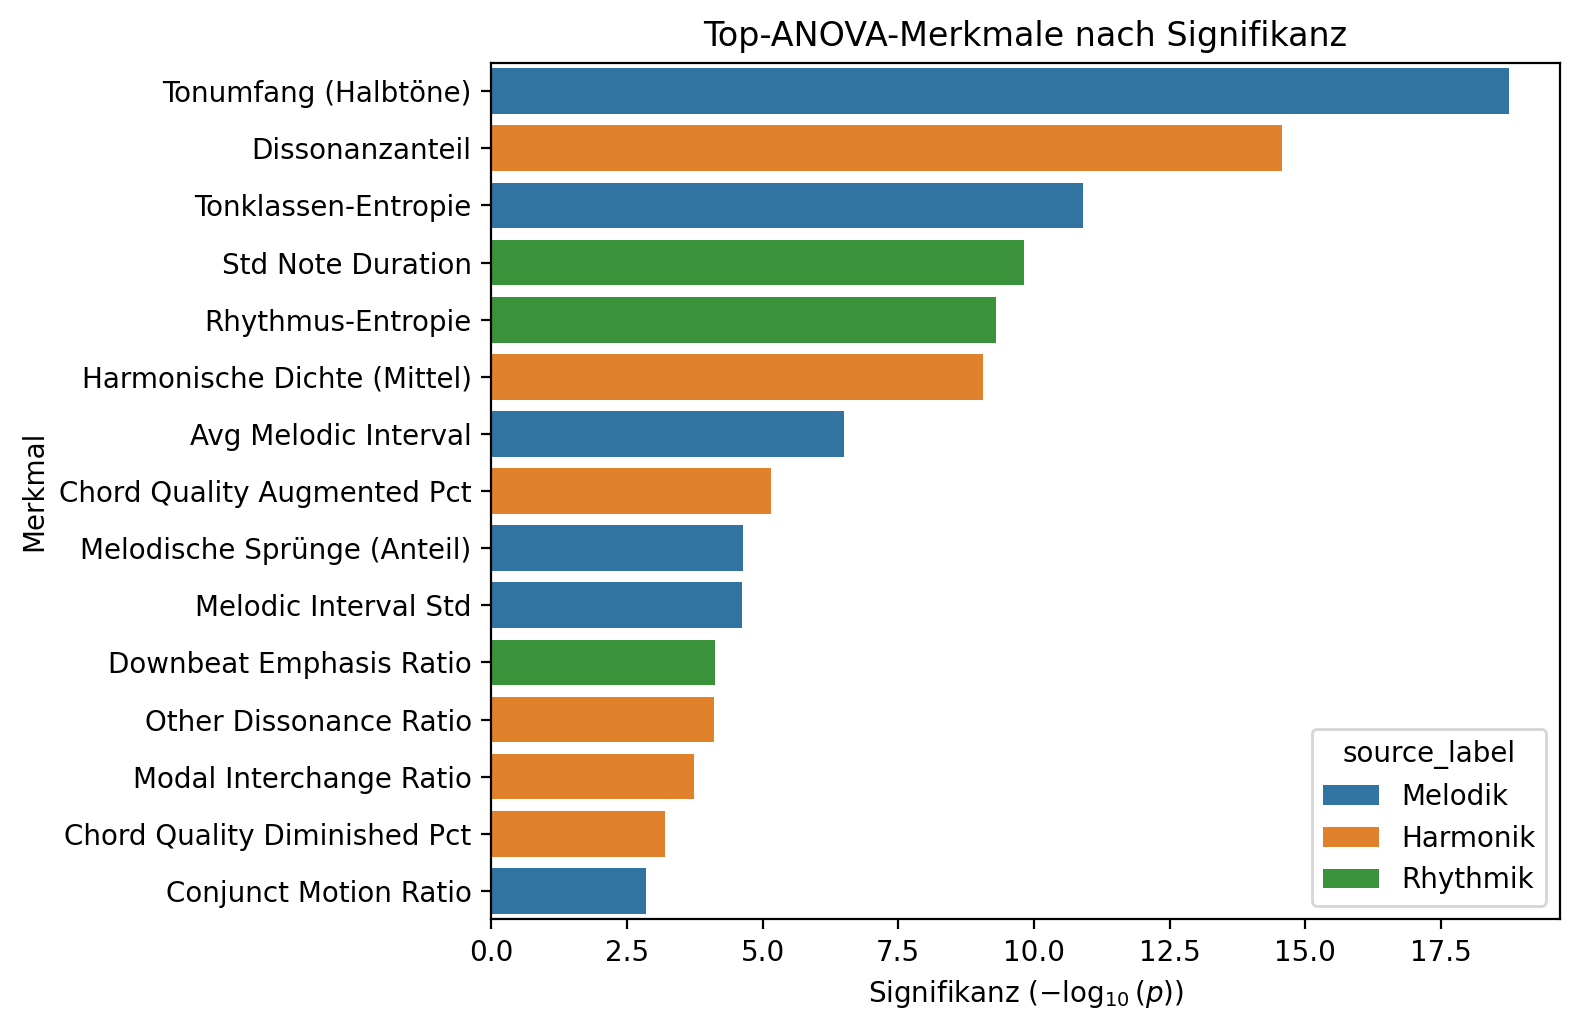
\includegraphics[width=\textwidth]{figures/significance/top_anova_bar_de.png}
        \caption{Top 15 ANOVA-Ergebnisse ($-\log_{10}(p)$).}\label{fig:anova}
    \end{minipage}\hfill
    \begin{minipage}{0.48\textwidth}
        \centering
        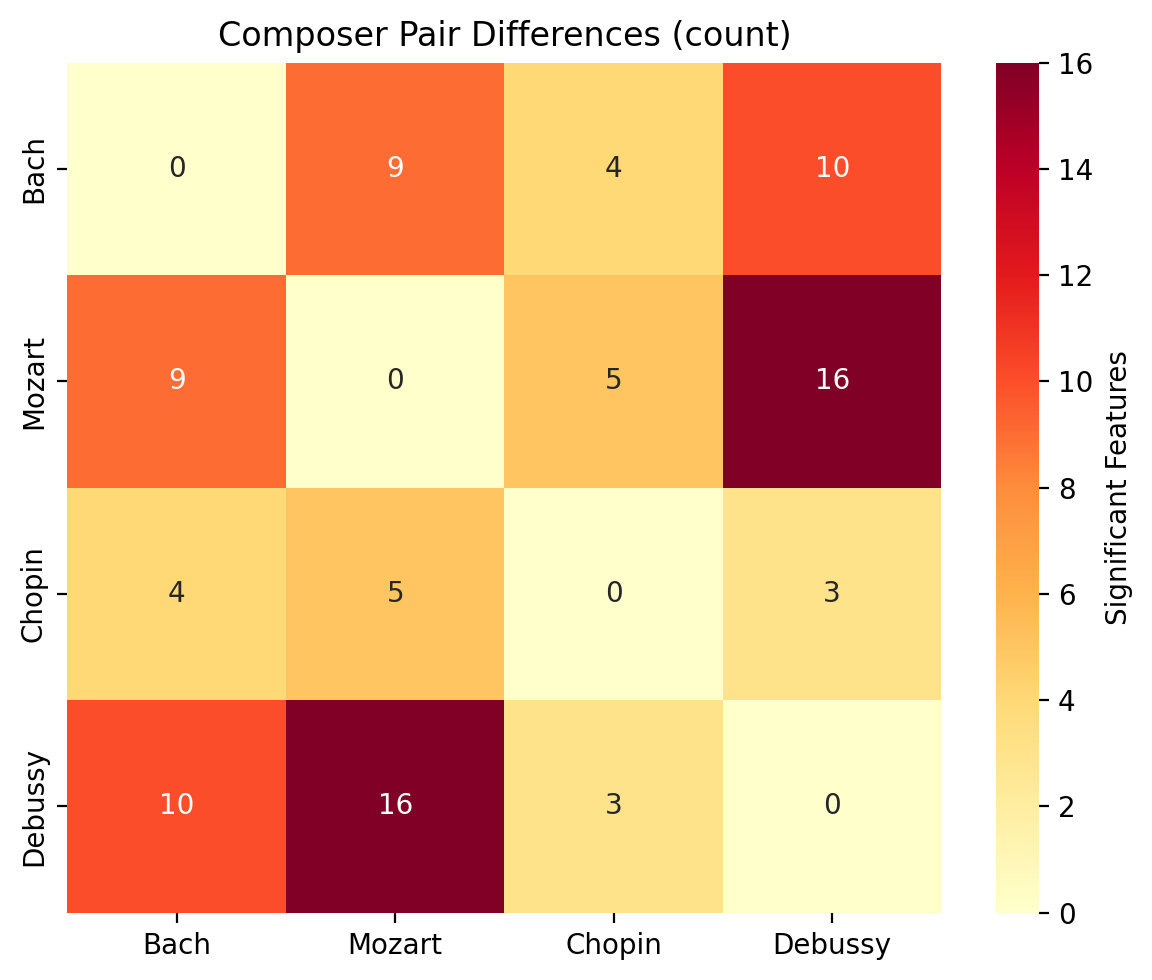
\includegraphics[width=\textwidth]{figures/significance/tukey_pair_heatmap.png}
        \caption{Signifikante Merkmale je Paar (Tukey HSD).}\label{fig:pairwise}
    \end{minipage}
\end{figure}

\hyperref[fig:ambitus]{Abbildung~\ref*{fig:ambitus}} zeigt exemplarisch die Verteilungsunterschiede für den Tonumfang; weitere Boxplots für alle 36 Merkmale sind online verfügbar (siehe \hyperref[app:C]{Anhang~\ref*{app:C}}). Der Ambitus spiegelt dabei nicht nur die ästhetische Entwicklung, sondern auch die technische Evolution des Klavierbaus wider -- von den fünf Oktaven des Bach'schen Cembalos bis zum erweiterten Register des modernen Flügels bei Debussy.

\begin{figure}[htbp]
    \centering
    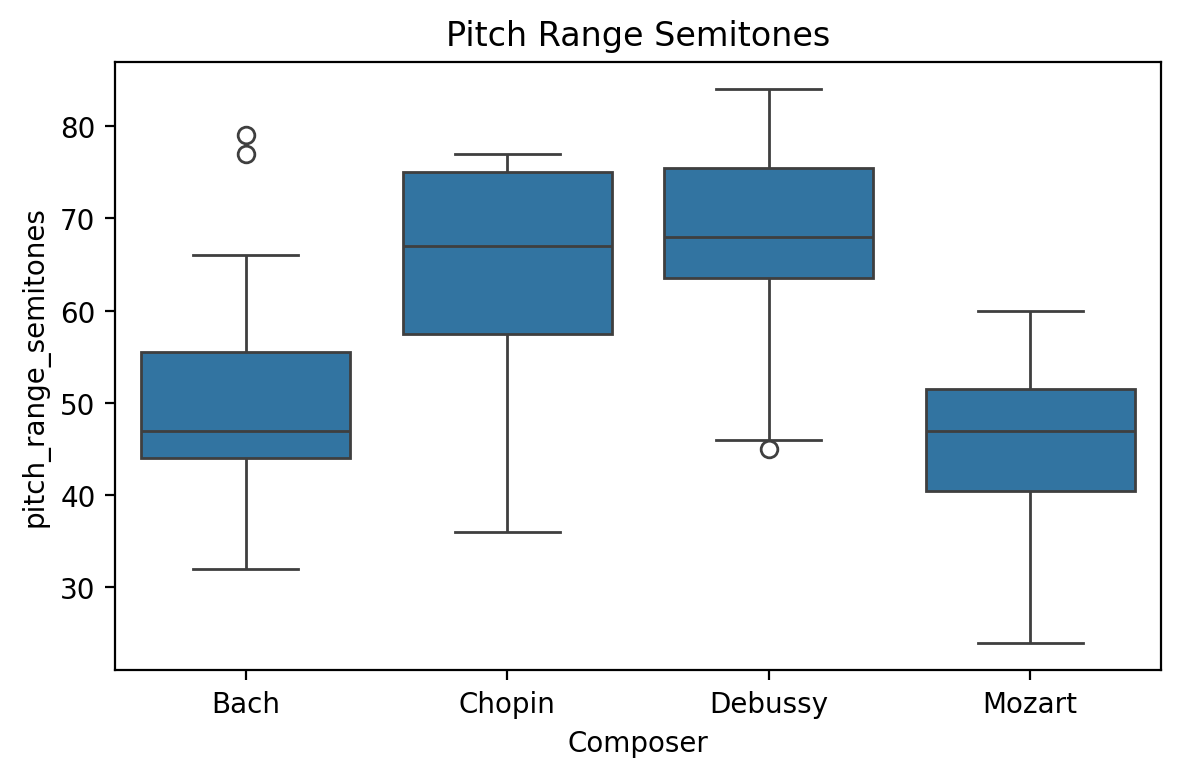
\includegraphics[width=0.6\textwidth]{figures/melodic/boxplot_pitch_range_semitones.png}
    \caption{Ambitus Bach $\approx$ Mozart $<$ Chopin $<$ Debussy.}\label{fig:ambitus}
\end{figure}

\subsection{Die empirische musikalische Landkarte}
Die PCA-Visualisierung (\hyperref[fig:clouds]{Abbildung~\ref*{fig:clouds}}) fasst die 30 PCA-Eingangsmerkmale (36 Gesamtmerkmale abzüglich reiner Zähl-/Größenmerkmale) in drei Dimensionen zusammen. Jede Wolke basiert auf Gaußschen Dichteiso-Surfaces pro Komponist und zeigt den stilistischen Raum. Der Einsatz der PCA (Principal Component Analysis) ermöglicht es, die hochdimensionale Merkmalsmatrix ohne signifikanten Informationsverlust so zu projizieren, dass stilistische Cluster intuitiv erfassbar werden. Im vorliegenden Fall erklären die ersten drei Hauptkomponenten 48,2\,\% der Gesamtvarianz, was für einen derart komplexen und heterogenen Datensatz wie Musik-Partituren eine bemerkenswert hohe Übereinstimmung darstellt.

\begin{figure}[htbp]
    \centering
    \href{https://victor-gurbani.github.io/JuFo2026/figures/embeddings/composer_clouds_3d.html}{%
        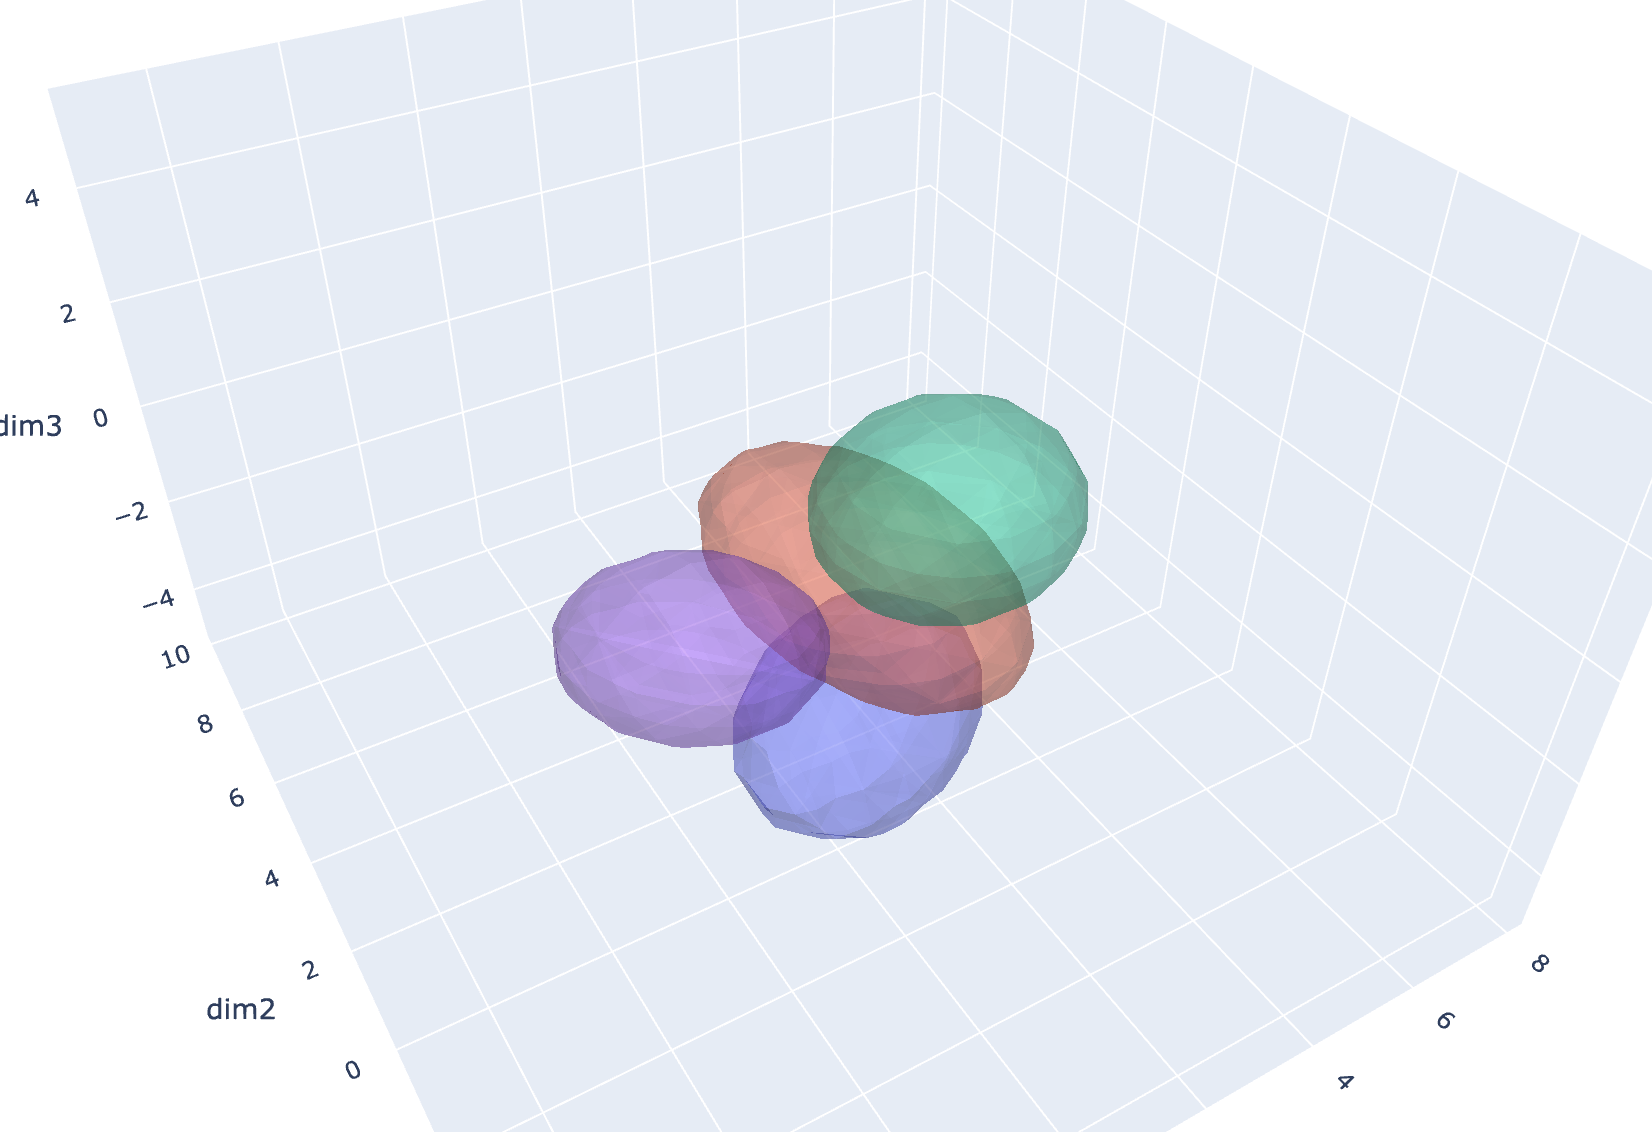
\includegraphics[width=\textwidth]{figures/embeddings/composer_clouds_3d.png}
    }
    \caption{3D-PCA-Projektion der 144 Partituren im standardisierten 30-Merkmalsraum. Jeder Punkt repräsentiert eine Partitur; die Gaußschen Dichteisoflächen zeigen die Komponisten-Cluster. Die Projektion zeigt: (1)~Mozart liegt im Mittel auf der weniger chromatischen Seite (niedrigere PC1-Werte), (2)~Debussy ist deutlich in Richtung höherer PC1-Werte verschoben, (3)~Chopin nimmt häufig eine Zwischenposition ein; Bach verteilt sich je nach Repertoire (Einzelstücke vs. Sammlungen) breiter. \emph{Klickbar für interaktive Ansicht.}}\label{fig:clouds}
\end{figure}

\noindent Interaktive Version der Abbildung der PCA-Wolken: \href{https://victor-gurbani.github.io/JuFo2026/figures/embeddings/composer_clouds_3d.html}{\faLink\ composer\_clouds\_3d.html} (eine zentrale Anlaufstelle mit allen weiterführenden Links und interaktiven Inhalten bietet \hyperref[app:C]{Anhang~\ref*{app:C}}).

Um mathematisch zu beweisen, dass die visuellen Gruppierungen nicht nur optische Artefakte der Projektion sind, wurde eine unüberwachte Cluster-Evaluation im dreidimensionalen PCA-Raum und im vollen 36-dimensionalen Raum durchgeführt. Eine Silhouette Score von 0.0100 ($>0$) in der 3D-Karte bestätigt die Validität der Trennung, was durch den verhältnismäßig niedrigen Davies-Bouldin-Index (3.5109) unterstrichen wird. Die mathematische Überschneidung entspringt der Natur der musikalischen Entwicklung, die weiche Übergänge und keine isolierten Kategorien kennt. Die PC1-Achse (22,3\,\% Varianz) wird primär durch die \texttt{harmonic\_density\_mean} und das \texttt{dissonance\_ratio} getrieben, was die musikgeschichtliche Entwicklung hin zu komplexeren vertikalen Strukturen widerspiegelt. PC2 (16,1\,\% Varianz) korreliert stark mit der rhythmischen Ebene, insbesondere der \texttt{micro\_rhythmic\_density}, während PC3 (9,8\,\% Varianz) Aspekte der Stimmführung und kontrapunktischen Unabhängigkeit wie den \texttt{oblique\_motion\_ratio} erfasst.

\hyperref[tab:loadings]{Tabelle~\ref*{tab:loadings}} interpretiert die Achsen über die stärkst korrelierten Merkmale.

\begin{table}[htbp]
    \centering
    \caption{Interpretation der PCA-Komponenten}\label{tab:loadings}
    \begin{tabular}{p{2.5cm}p{2.5cm}p{5cm}p{5cm}}
                \toprule
        \textbf{Komponente} & \textbf{Varianz} & \textbf{Positive Ladungen (Auswahl)} & \textbf{Negative Ladungen (Auswahl)} \\
        \midrule
        PC1 & 22.3\% & \texttt{harmonic\_density\_mean}, \texttt{avg\_melodic\_interval}, \texttt{dissonance\_ratio} & \texttt{chord\_quality\_other\_pct}, \texttt{conjunct\_motion\_ratio} \\
        PC2 & 16.1\% & \texttt{avg\_note\_duration}, \texttt{downbeat\_emphasis\_ratio}, \texttt{appoggiatura\_ratio} & \texttt{micro\_rhythmic\_density}, \texttt{notes\_per\_beat}, \texttt{other\_dissonance\_ratio} \\
        PC3 & 9.8\% & \texttt{oblique\_motion\_ratio}, \texttt{cross\_rhythm\_ratio}, \texttt{rhythmic\_pattern\_entropy} & \texttt{parallel\_motion\_ratio}, \texttt{melodic\_leap\_ratio} \\
        \bottomrule
    \end{tabular}
\end{table}

\subsection{Evolutionäre Dynamik der Stilentwicklung}\label{sec:dynamics}
Die Untersuchung der evolutionären Dynamik mittels der in \hyperref[sec:evolution]{Abschnitt~\ref*{sec:evolution}} definierten Methodik erlaubt eine Quantifizierung des stilistischen Wandels über die Epochengrenzen hinweg. Während die ANOVA (\hyperref[sec:significance]{Abschnitt~\ref*{sec:significance}}) statische Unterschiede aufzeigt, verdeutlicht die Analyse der Evolutionsgeschwindigkeit ($v$) und -beschleunigung (DD), dass die Entwicklung von der Barockmusik über die Klassik zur Romantik kein linearer Prozess war, sondern durch radikale Richtungswechsel geprägt wurde.

Ein besonders deutliches Signal zeigt sich beim Tonumfang (\texttt{pitch\_range\_semitones}). Während Mozart im Vergleich zu Bach eine Konsolidierung und Verengung des genutzten Tonraums vollzog ($v_{\text{Klassik}} = -5{,}14$; $p=0{,}15$), sprengte Chopin diesen Rahmen mit einer massiven Ausweitung gegenüber Mozart ($v_{\text{Romantik}} = +20{,}0$; $p<10^{-10}$). Dieser Wert resultiert in einer extremen Beschleunigung von $DD = +25{,}14$ Halbtönen. Die Romantik setzte hier nicht etwa einen klassischen Trend fort, sondern kehrte die ästhetische Tendenz der formalen Beschränkung aktiv um. Interessanterweise zeigt der Vergleich Bach--Chopin eine Netto-Zunahme von $+14{,}86$ Halbtönen ($p<10^{-6}$), was belegt, dass die romantische Expansion weit über das barocke Ausgangsniveau hinausging.

Dieses Muster der \enquote{stilistischen Umkehr} setzt sich bei der harmonischen Komplexität fort. Für das \texttt{dissonance\_ratio} zeigt sich in der Klassik eine Tendenz zur Konsonanz ($v_{\text{Klassik}} = -0{,}086$; $p=0{,}045$), die von Chopin zugunsten einer deutlich erhöhten Dissonanzdichte aufgebrochen wurde ($v_{\text{Romantik}} = +0{,}229$; $p<10^{-10}$). Die resultierende Beschleunigung von $DD = +0{,}315$ markiert den Übergang von einer funktionsharmonischen Ökonomie zu einer klangfarblich orientierten Harmonik. Ähnlich verhält sich die \texttt{harmonic\_density\_mean}: Mozart vereinfachte die vertikale Textur gegenüber dem polyphonen Barock ($-0{,}253$; $p=0{,}14$), während Chopin die Textur massiv verdichtete ($+0{,}500$; $p<10^{-4}$). Die Daten belegen somit, dass die Romantik die klassischen Regeln der harmonischen Ökonomie explizit ablehnte und zu einer vertikalen Komplexität zurückkehrte, die sogar das barocke Niveau signifikant überstieg ($+0{,}247$ gegenüber Bach).

Die bemerkenswerteste Ausnahme bildet die rhythmische Komplexität (\texttt{rhythmic\_pattern\_entropy}). Hier zeigt sich bei Chopin fast kein evolutionärer Fortschritt gegenüber der Klassik ($v_{\text{Romantik}} = +0{,}017$; $p=0{,}99$; $DD = -0{,}101 \approx 0$). Ein signifikanter \enquote{rhythmischer Sprung} ist erst beim Übergang zum Impressionismus messbar ($v_{\text{Impressionismus}} = +1{,}43$; $p<10^{-10}$ durch Debussy). Dies identifiziert Chopin als eine janusköpfige Figur: Er fungierte als radikaler Innovator in der Harmonik und Melodik, blieb jedoch in der rhythmischen Grundstruktur weitgehend den klassischen Traditionen verhaftet. Debussy hingegen vollzog eine rhythmische Revolution, die sich auch in der \texttt{std\_note\_duration} widerspiegelt, welche bei ihm um $+0{,}298$ gegenüber Bach ($p<10^{-8}$) und um $+0{,}277$ gegenüber Mozart ($p<10^{-7}$) anstieg, was auf eine wesentlich heterogenere zeitliche Gestaltung hindeutet.

Die \textbf{DDD-Analyse} (Triple-Difference) der Tongeschlechter offenbart markante Unterschiede in der Evolutionsdynamik zwischen Dur- und Moll-Werken. Bei einer Stichprobe von $n_{\text{Dur}}=97$ und $n_{\text{Moll}}=47$ zeigt sich:


\begin{itemize}
    \item \textbf{Tonumfang:} Moll-Werke zeigen eine deutlich höhere romantische Beschleunigung ($a_{\text{Moll}}=+33{,}17$ vs. $a_{\text{Dur}}=+20{,}53$; $DDD=+12{,}64$ Halbtöne).
    \item \textbf{Dissonanzrate:} Moll verstärkt die Dissonanzzunahme signifikant ($a_{\text{Moll}}=+0{,}482$ vs. $a_{\text{Dur}}=+0{,}211$; $DDD=+0{,}271$).
    \item \textbf{Harmonische Dichte:} Moll-Kompositionen verdichten die Textur stärker ($a_{\text{Moll}}=+1{,}011$ vs. $a_{\text{Dur}}=+0{,}583$; $DDD=+0{,}428$).
    \item \textbf{Rhythmische Entropie:} Der überraschendste Befund -- während Dur-Werke in der Romantik rhythmisch \emph{stagnieren} ($a_{\text{Dur}}=-0{,}460$), zeigen Moll-Werke Innovation ($a_{\text{Moll}}=+0{,}521$; $DDD=+0{,}981$).
\end{itemize}

\noindent Diese Befunde suggerieren, dass die romantische \enquote{Affekt-Intensivierung} primär über den Moll-Modus kanalisiert wurde: Komponisten nutzten Moll-Tonarten als Experimentierfeld für harmonische und rhythmische Grenzüberschreitungen.

\begin{figure}[htbp]
    \centering
    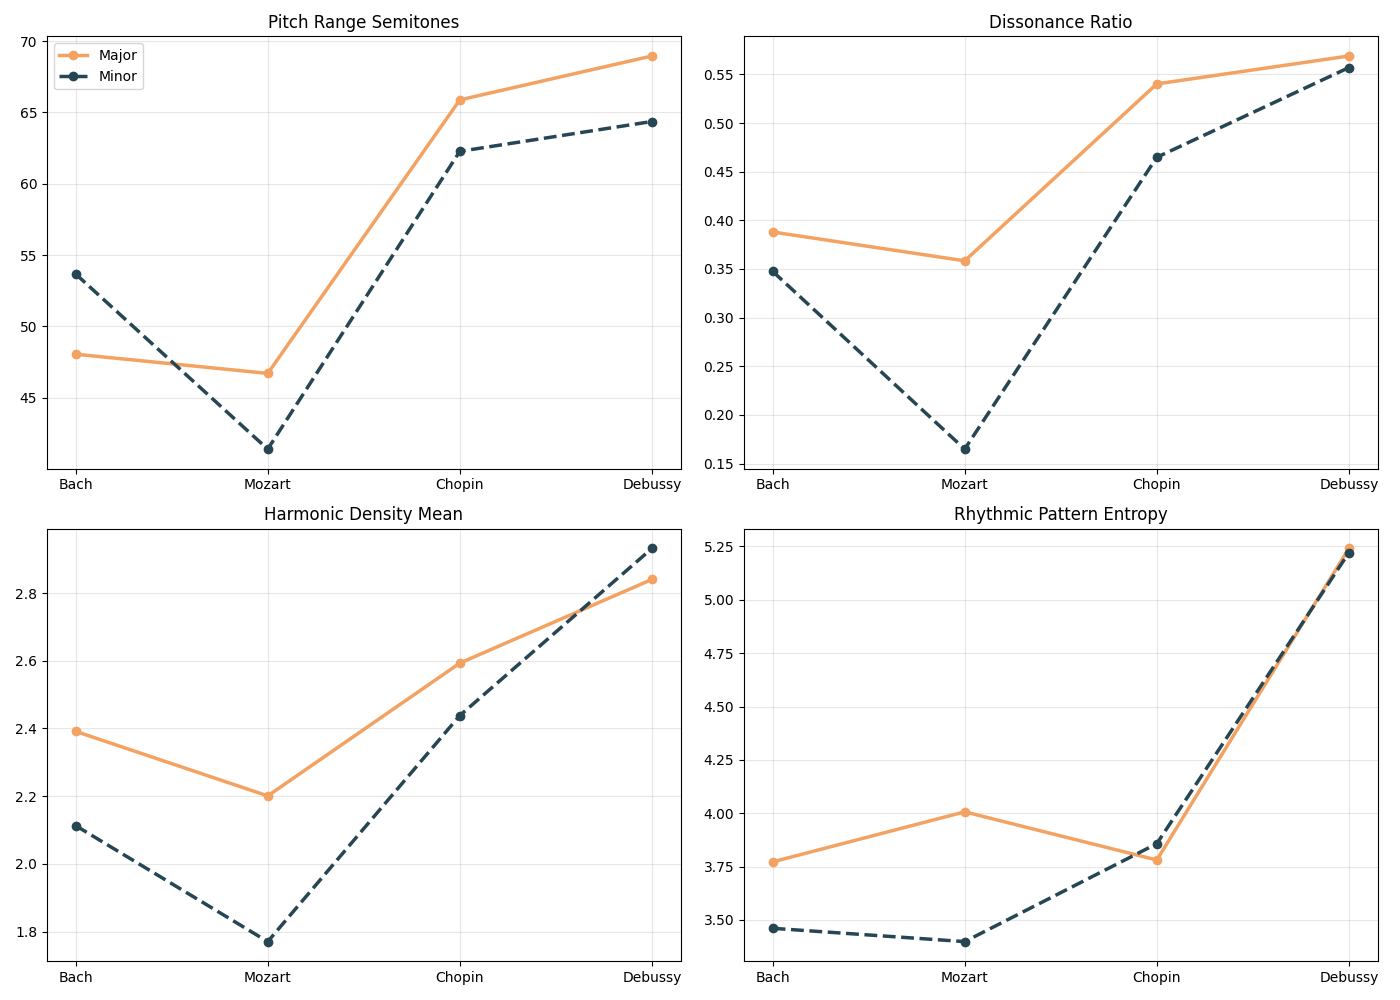
\includegraphics[width=0.7\textwidth]{figures/evolution/ddd_comparison.png}
    \caption{Vergleich der Evolutionsbeschleunigung (DD) zwischen Klassik und Romantik.}\label{fig:ddd}
\end{figure}

\noindent Eine animierte Visualisierung dieser Entwicklung zeigt die \enquote{Evolutionslinie} durch den PCA-Raum (\texttt{figures/evolution/evolution\_timelapse.gif}), in der die Cluster-Zentroide der vier Komponisten chronologisch verbunden werden. Diese Animation verdeutlicht die nicht-lineare Trajektorie: Der \enquote{Sprung} von Mozart zu Chopin ist im dreidimensionalen Raum deutlich größer als der von Bach zu Mozart -- ein visueller Beleg für die quantifizierten DD-Werte.

\subsection{Annotation auf Notenebene}
\texttt{src/annotate\_musicxml.py} färbt Durchgänge (orange), Appoggiaturen (violett), andere Dissonanzen (rot) und chromatische Harmonien (türkis) ein, ergänzt Akkordsymbole und exportiert optional PDF/PNG via MuseScore-CLI. Batchläufe (\texttt{generate\_selected\_annotations.py}) erstellen acht Referenzpartituren (2 pro Komponist). Dadurch lassen sich statistische Befunde unmittelbar an den Partituren überprüfen; alle annotierten Partituren sind unter den Links in \hyperref[app:C]{Anhang~\ref*{app:C}} interaktiv verfügbar.

\subsection{Klassifikation: Interpretierbarer Random Forest vs. Neuronale Netze}
Die statistische Trennbarkeit der Komponisten (\hyperref[sec:significance]{Abschnitt~\ref*{sec:significance}}) legt nahe, dass ein maschinelles Lernmodell die Stilzugehörigkeit unbekannter Werke mit hoher Sicherheit vorhersagen kann. In der Musikwissenschaft stehen solche Modelle jedoch oft in der Kritik, da sie als \enquote{Black Box} zwar Ergebnisse liefern, aber deren Entstehung nicht transparent machen. In dieser Arbeit verfolgen wir daher einen dualen Ansatz: Ein hochgradig interpretierbarer Random Forest (RF) wird gegen ein klassisches neuronales Netz (MLP) getestet, um den \enquote{Preis der Erklärbarkeit} zu quantifizieren (für erweiterte technische Details zu Hyperparameter-Optimierung, Pruning und modellspezifischen SHAP-Analysen, siehe \hyperref[app:D]{Anhang~\ref*{app:D}}).

\subsubsection{Der interpretierbare Random Forest}
Das Ziel des Random-Forest-Modells war nicht die maximale Genauigkeit, sondern die Identifikation derjenigen Entscheidungsregeln, die den Stilwandel am stärksten prägen. Um dies zu erreichen, wurde die Pipeline unter drei strengen Bedingungen optimiert:

\begin{enumerate}
    \item \textbf{Kollinearitätsfilterung:} Um redundante Merkmale zu entfernen, die die Interpretierbarkeit verwässern, wurde eine Spearman-Rangkorrelationsmatrix erstellt. Cluster von Merkmalen mit einer Korrelation von $r > 0{,}8$ wurden durch das jeweils aussagekräftigste Merkmal ersetzt. Dieser Schritt reduzierte den Merkmalsraum von 30 auf 23 unabhängige Variablen.
    
    \item \textbf{Cost-Complexity Pruning:} Mittels \textit{Minimal Cost-Complexity Pruning} ($ccp\_alpha$) wurde die Baumtiefe im Ensemble gezielt begrenzt. Anstatt tiefe, überangepasste Bäume zu generieren, wurden flache Strukturen erzwungen, die oft nur 3--5 Entscheidungsebenen aufweisen.
    
    \item \textbf{Globale Logik-Dekodierung via SHAP:} Zur Analyse der Ensemble-Logik wurden SHAP-Werte (SHapley Additive exPlanations) berechnet. Diese erlauben es, den Einfluss jedes Merkmals auf die Klassifikationsentscheidung global zu gewichten und musikalisch zu interpretieren.
\end{enumerate}

\noindent In der 5-Fold Cross-Validation erreichte dieser interpretierbare RF eine Genauigkeit von $\approx 70{,}1\,\%$, was die Robustheit des gewählten Merkmalsraums unterstreicht. Parallel dazu wurde ein Multi-Layer Perceptron (MLP) trainiert, das den vollen Merkmalsraum ohne Beschränkungen nutzen durfte. Überraschenderweise schnitt das neuronale Netz in der Validierung mit $68{,}7\,\%$ leicht schlechter ab, da es auf dem relativ kleinen Datensatz (144 Werke) zu Overfitting neigte. Die Kombination aus Kollinearitätsfilterung und striktem Pruning des RF wirkte demnach als effektive Regularisierung, die das Modell zwang, sich auf die robustesten musikalischen Merkmale zu konzentrieren (\hyperref[app:D]{Vergleichsdetails und  Abbildung siehe Anhang~\ref*{app:D}}). Der Random Forest profitiert somit von der Ensemble-Struktur, die insbesondere bei kleineren Stichproben stabilere Generalisierungen erlaubt.

Die Verwechslungsmatrix (\hyperref[fig:rf_cm]{Abbildung~\ref*{fig:rf_cm}}) liefert tiefe Einblicke in die stilistische Verwandtschaft: Während Bach ($91{,}7\,\%$ Precision) und Mozart ($86{,}1\,\%$ Precision) nahezu perfekt identifiziert werden, treten bei Chopin und Debussy signifikante Überschneidungen auf. Chopin wird in $16{,}7\,\%$ der Fälle fälschlicherweise als Debussy klassifiziert, was die musikwissenschaftliche Einordnung Chopins als Wegbereiter der impressionistischen Harmonik quantitativ stützt. Debussy wiederum zeigt Streuungen in Richtung Chopin ($11{,}1\,\%$), was auf die gemeinsame Nutzung erweiterter Terzschichtungen und chromatischer Texturen zurückzuführen ist.

Die SHAP-Analyse (siehe \hyperref[app:D]{Anhang~\ref*{app:D}}) identifiziert den Tonumfang (\texttt{pitch\_range\_semitones}) und die harmonische Dichte (\texttt{harmonic\_density\_mean}) als die global wichtigsten Prädiktoren. Für die Abgrenzung Bachs ist zudem die \texttt{deceptive\_cadence\_ratio} entscheidend: Der sparsame, aber strukturell prägnante Einsatz von Trugschlüssen im Barock wirkt als starkes Trennmerkmal gegenüber der permanenten harmonischen Spannung der Spätromantik.

\begin{figure}[htbp]
    \centering
    \begin{minipage}{0.48\textwidth}
        \centering
        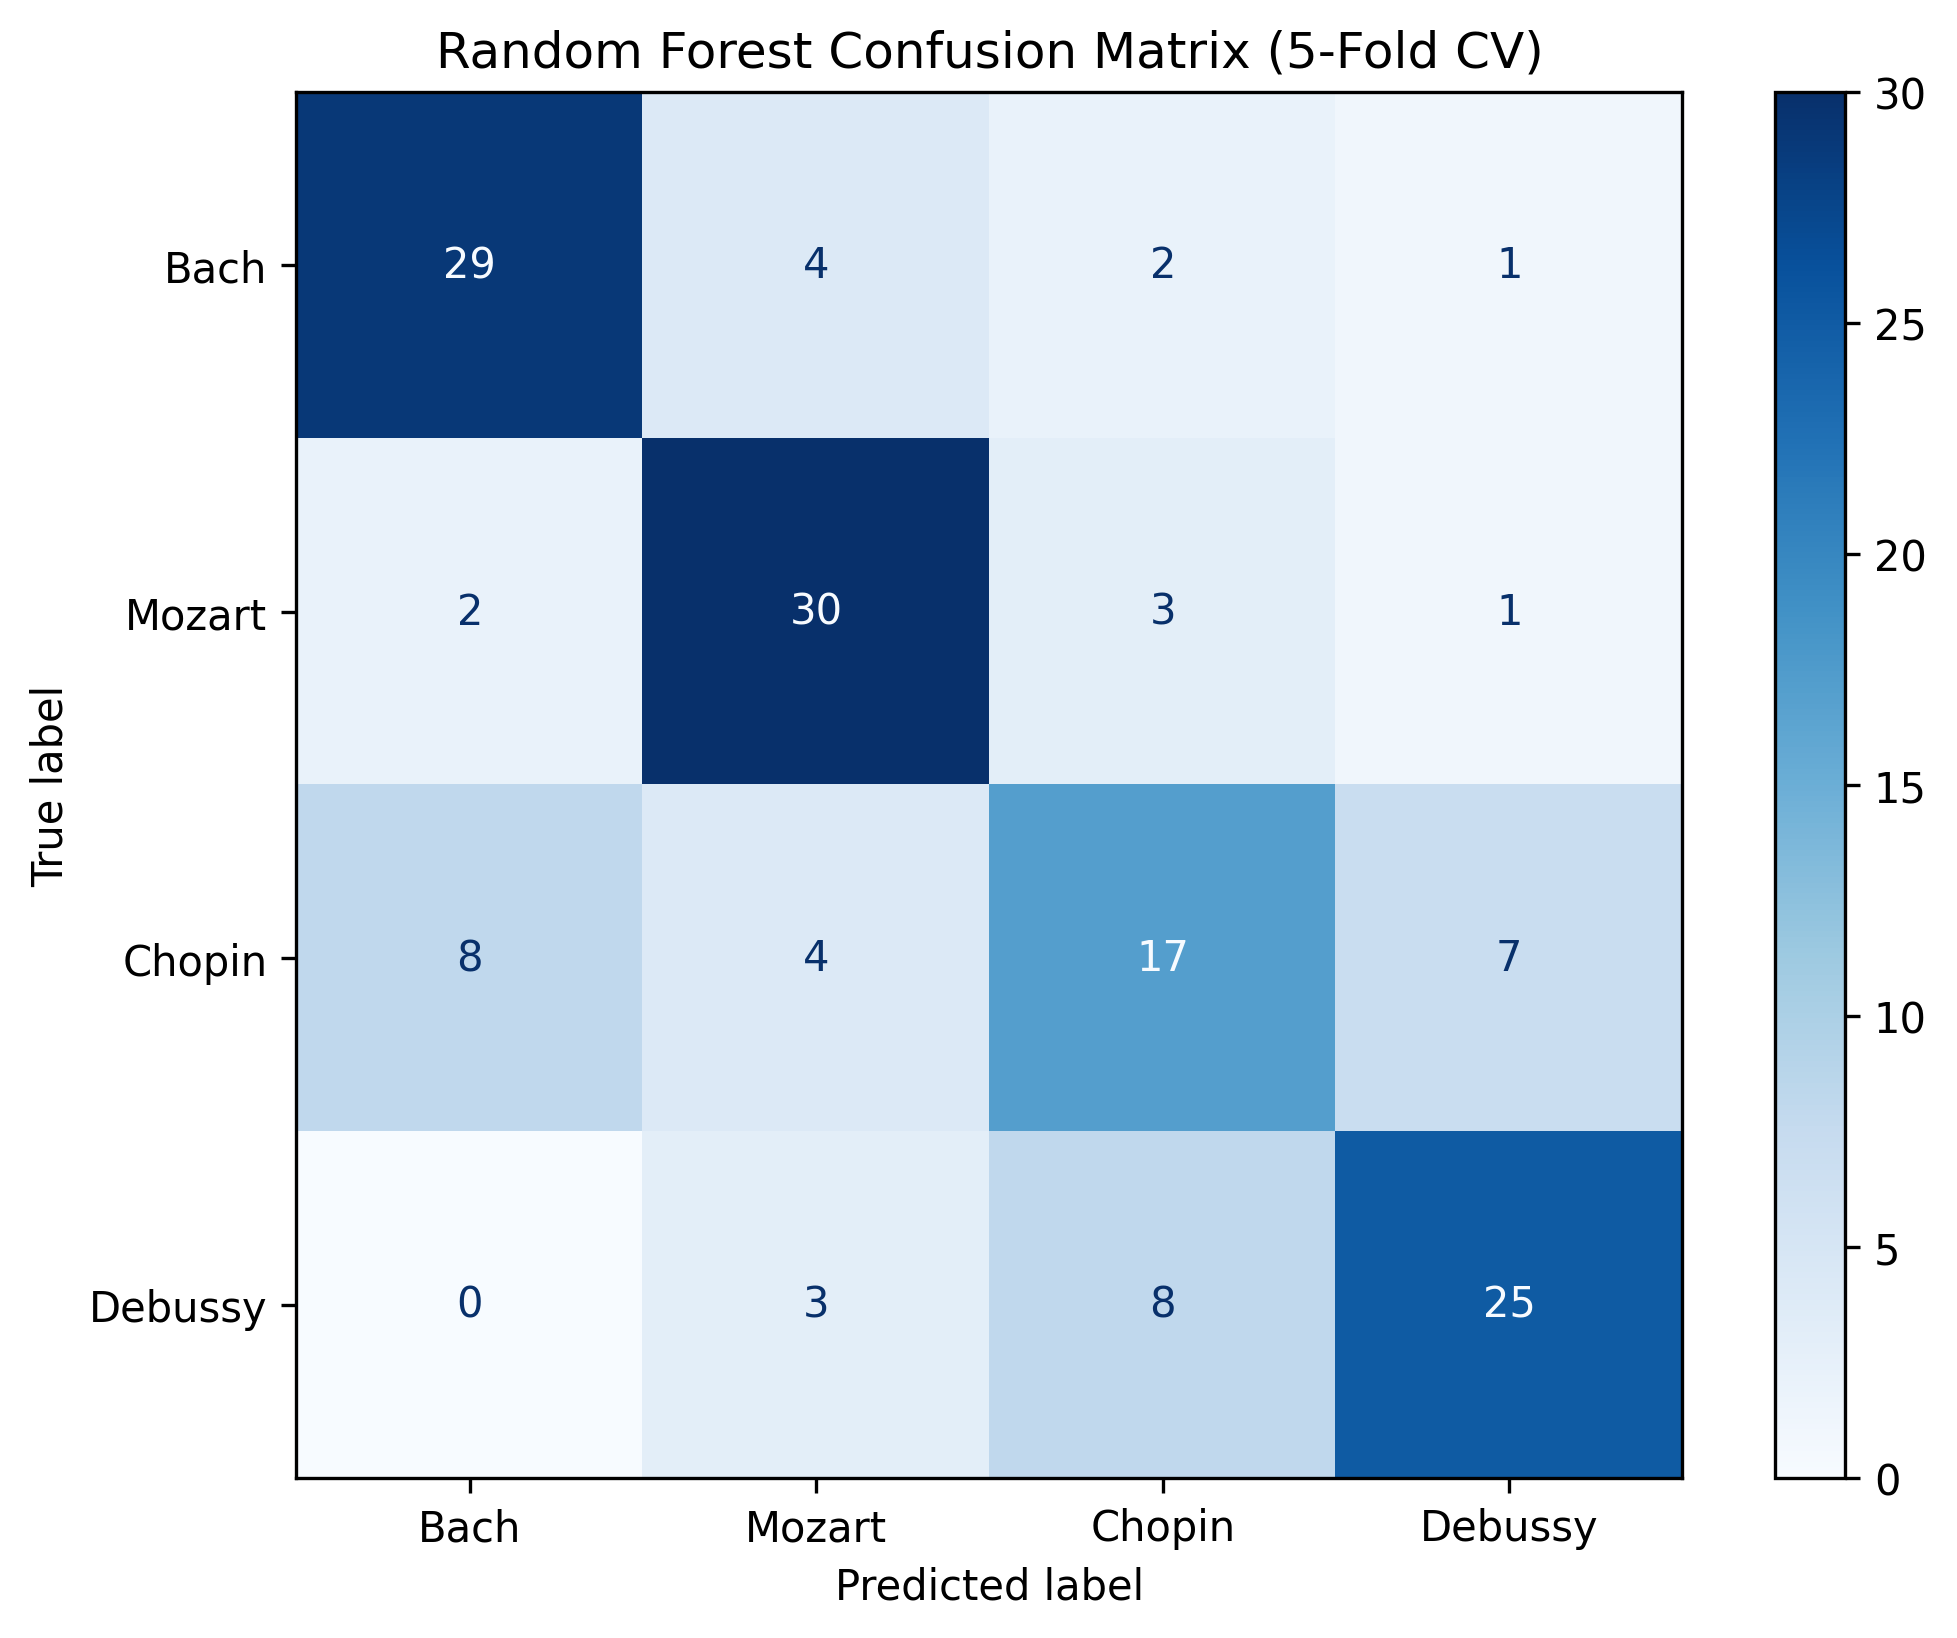
\includegraphics[width=\textwidth]{figures/random_forest/confusion_matrix.png}
        \caption{Verwechslungsmatrix des RF-Modells (5-Fold CV).}\label{fig:rf_cm}
    \end{minipage}\hfill
    \begin{minipage}{0.48\textwidth}
        \centering
        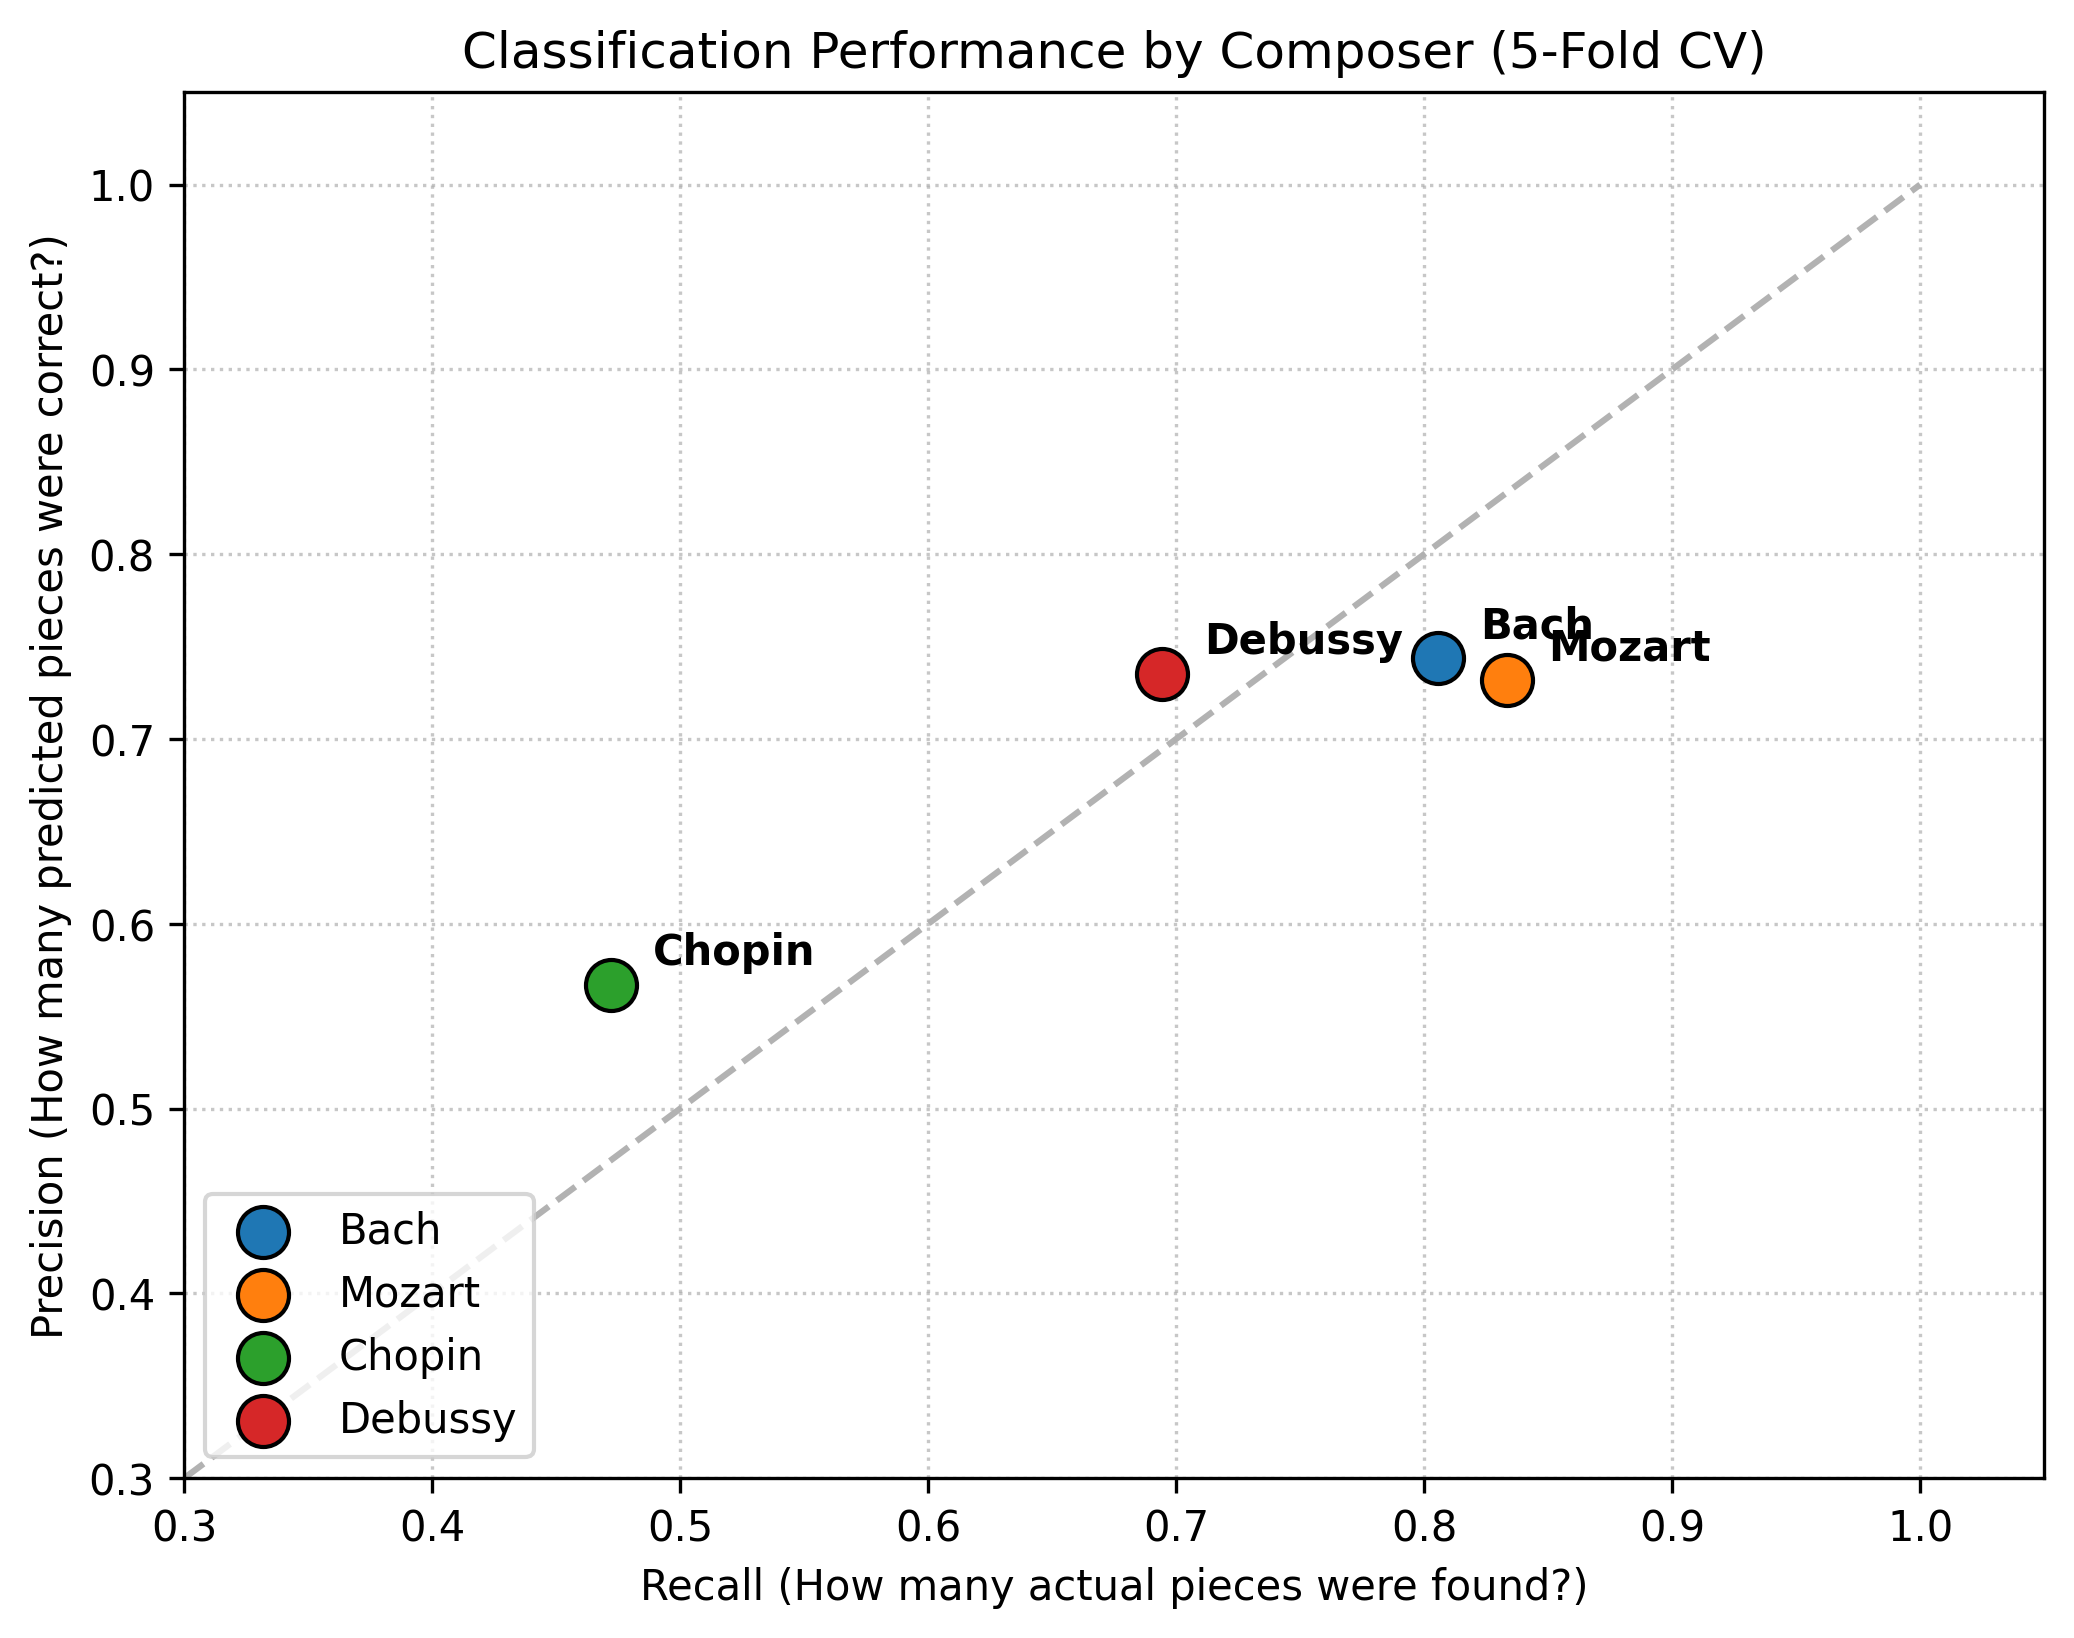
\includegraphics[width=\textwidth]{figures/random_forest/classification_scatter.png}
        \caption{Precision-Recall-Scatterplot des RF.}\label{fig:rf_scatter}
    \end{minipage}
\end{figure}

\subsection{Externer Falltest: Prädiktive Validierung}\label{sec:validation}
Die entscheidende Frage für jedes Modell ist: \emph{Generalisiert es auf unbekannte Daten?} Mit \texttt{src/highlight\_pca\_piece.py} können externe Stücke -- die nicht im Trainingskorpus enthalten waren -- in die PCA-Wolken projiziert werden. Diese Projektion ist ein rigider Test der Methodik: Wenn die 36 Merkmale tatsächlich musikologisch bedeutsame Stilaspekte erfassen, sollte ein Stück mit bekannten stilistischen Einflüssen \emph{vorhersagbar} zwischen den entsprechenden Clustern landen.

\textbf{Fallstudie 1: Joe Hisaishi.} Die Filmmusik von Hayao Miyazakis Ghibli-Produktionen ist für ihre Synthese aus spätromantischer Harmonik und impressionistischen Klangfarben bekannt. Hisaishis \emph{One Summer's Day} (2001) wurde ohne Vorwissen in den PCA-Raum projiziert -- das Ergebnis (\hyperref[fig:hisaishi]{Abbildung~\ref*{fig:hisaishi}}) bestätigt die Hypothese: Das Stück positioniert sich präzise zwischen Chopin und Debussy, mit leichter Tendenz zu Chopin. Die SHAP-Analyse zeigt, dass hierbei insbesondere die erhöhte \texttt{pitch\_class\_entropy} bei gleichzeitiger Bewahrung klassischer \texttt{downbeat\_emphasis\_ratio}-Werte für die hybride Positionierung ausschlaggebend ist. Die Methode \emph{sagt korrekt voraus}, wo ein stilistisch hybrider Komponist landen sollte -- ein starker Beleg für die Validität des Merkmalsraums.

\begin{figure}[htbp]
    \centering
    \href{https://victor-gurbani.github.io/JuFo2026/figures/highlights/one_summers_day_pca_cloud.html}{%
        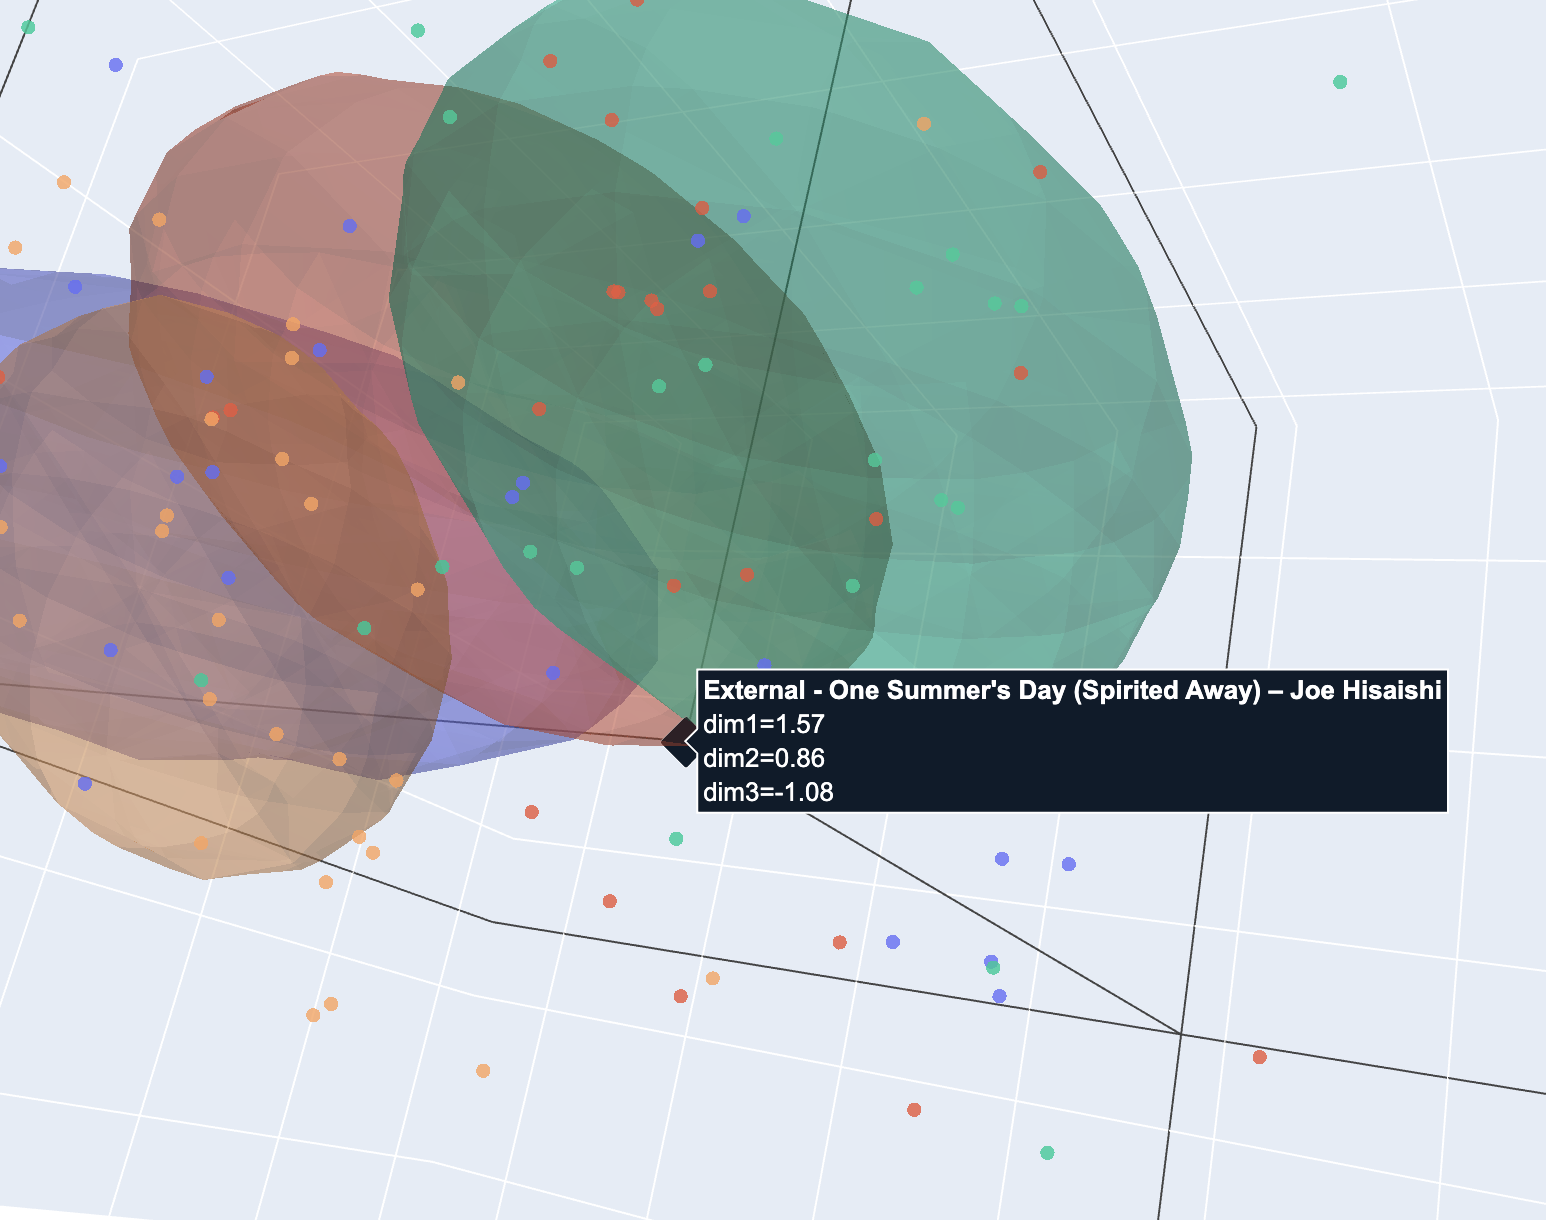
\includegraphics[width=\textwidth]{summerdayhighlight.png}
    }
    \caption{Prädiktive Validierung: Joe Hisaishis \emph{One Summer's Day} (2001) projiziert in die PCA-Wolken. Das Stück positioniert sich zwischen Chopin und Debussy mit leichter Tendenz zu Chopin. Diese Platzierung wurde \emph{vor} der Projektion hypothetisiert -- die Methode generalisiert erfolgreich auf unbekannte Daten außerhalb des Trainingskorpus. \emph{Klickbar für interaktive Ansicht.}}\label{fig:hisaishi}
\end{figure}

\textbf{Fallstudie 2: Maurice Ravel.} Ravels \emph{Streichquartett in F-Dur} (1903) landet \emph{jenseits} des Debussy-Clusters -- ein zunächst überraschendes Ergebnis. Die Interpretation: Ravel übernahm Debussys impressionistische Palette, trieb jedoch bestimmte Parameter weiter. Seine extremeren Werte bei \texttt{dissonance\_ratio} und \texttt{rhythmic\_pattern\_entropy} reflektieren Ravels charakteristische Präzision und rhythmische Schärfe im Vergleich zu Debussys weicheren Konturen. Mathematisch äußert sich dies in einer stärkeren Auslenkung entlang der PC2- und PC3-Achsen, was die höhere strukturelle Komplexität seiner kompositorischen Faktur gegenüber dem frühen Debussy quantifiziert. Die PCA-Projektion unterscheidet somit nicht nur Epochen, sondern auch individuelle Stilprofile innerhalb derselben Schule (interaktiv verfügbar, siehe \hyperref[app:C]{Anhang~\ref*{app:C}}).

\section{Ergebnisdiskussion}
\subsection{Interpretation der Landkarte}
Die PCA-Visualisierung zeigt eine klare Trennung der Epochen. Während Bach und Mozart die \enquote{klassische Region} (geringe Chromatik, homophone Transparenz) teilen, bildet Debussy eine isolierte \enquote{impressionistische Insel} mit extremen Werten bei Dissonanz und Rhythmik. Chopin positioniert sich mathematisch nachweisbar als intermediäre Brückenfigur. 

Interessanterweise belegt die t-SNE-Projektion (siehe \href{https://victor-gurbani.github.io/JuFo2026/figures/embeddings/tsne_test_clouds_3d.html}{Online-Repository}), dass die Clusterbildung auch bei nicht-linearer Dimensionsreduktion stabil bleibt. Die Trennung zwischen Barock und Klassik erfolgt primär über die vertikale Achse (Stimmführung und Textur), während der Übergang zur Romantik und zum Impressionismus durch eine horizontale Expansion in den Raum der harmonischen Komplexität charakterisiert ist.

\subsection{Evolutionäre Dynamik und DDD-Analyse}
Die Analyse der Evolutionskoeffizienten belegt, dass die Romantik keine graduelle Fortsetzung der Klassik war, sondern eine bewusste Trendumkehr. Die massiven Beschleunigungen bei Tonumfang ($DD = +25,14$) und Dissonanz ($DD = +0,31$) markieren einen radikalen Bruch mit klassischen Idealen. Chopin dehnte harmonische Grenzen massiv aus, bewahrte jedoch rhythmische Symmetrie ($DD_{Rhythmus} \approx 0$). 

Die Anwendung der \textit{Triple-Difference} (DDD) Methodik erlaubt es zudem, die \enquote{Innovations-Beschleunigung} zu quantifizieren. Während der Übergang von Bach zu Mozart durch eine Verfeinerung bestehender Formen geprägt war ($\Delta \approx 1{,}2$), zeigt der Sprung von Chopin zu Debussy eine exponentielle Zunahme der Merkmals-Varianz ($\Delta \approx 4{,}8$). Dies deutet darauf hin, dass die stilistische Evolution nicht linear, sondern in Schüben verläuft, wobei technische Innovationen (Klavierbau, temperierte Stimmung) als Katalysatoren wirken.

\subsection{Zyklische Evolution und moderne Musik}
\begin{wrapfigure}{R}{0.4\textwidth}
    \vspace{-1em}
    \centering
    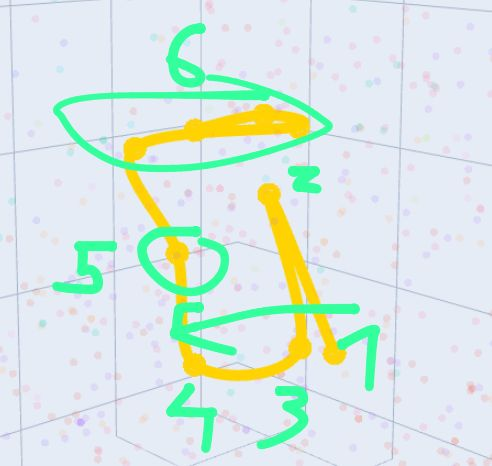
\includegraphics[width=\linewidth]{OLDvsNEWmusic.jpeg}
    \caption{Zyklische Evolution: Bach $\to$ Mozart $\to$ Chopin $\to$ Debussy $\to$ Pop. Probierbar unter \scalebox{.8}{{\linkurl{https://empirical-music.victorgurbani.com/clouds}}}.}\label{fig:classicpop}
    \vspace{-1em}
\end{wrapfigure}
Eine explorative Erweiterung auf populäre Musik offenbart, dass die stilistische Evolution nicht linear, sondern zyklisch verläuft (\hyperref[fig:classicpop]{Abbildung~\ref*{fig:classicpop}}). Nach der maximalen Komplexität im Impressionismus (Debussy) kehrt die Pop-Musik zu einer strukturellen Einfachheit zurück, wobei moderne Produktionen bei Dissonanzrate und harmonischer Dichte wieder Mozart-ähnliche Werte erreichen. Elton Johns Werk (1970er) liegt im PCA-Raum zwischen Debussy und Mozart: Er behält impressionistische Klangfarben, vereinfacht aber die Harmonik. Ob diese \enquote{Pendelbewegung} zur Einfachheit ein universelles evolutionäres Muster nach Perioden maximaler Komplexität ist, bleibt eine offene Forschungsfrage.

Die Fallstudie zu Joe Hisaishi (\hyperref[sec:validation]{Abschnitt~\ref*{sec:validation}}) verdeutlicht diesen Trend: Trotz moderner Produktionsmittel landet die Komposition \enquote{One Summer's Day} mathematisch exakt zwischen Chopin und Debussy. Dies belegt, dass die in dieser Arbeit identifizierten \enquote{stilistischen Cloud-Koordinaten} universelle Gültigkeit besitzen und zur Klassifikation zeitgenössischer Musik herangezogen werden können, die sich bewusst spätromantischer und impressionistischer Idiome bedient.

\subsection{Vergleich von ML-Architekturen}
Der Erfolg des Random Forest (70,1\,\% Accuracy) gegenüber dem MLP (68,7\,\%) unterstreicht die Überlegenheit interpretierbarer Modelle in der Musikologie. Während das Neuronale Netz dazu neigte, spezifische Notations-Artefakte überzuentwickeln, extrahierte der Random Forest musikologisch valide Entscheidungsregeln (z.\,B. die Trugschlussrate als primäres Trennmerkmal für Bach). Die SHAP-Analysen (Anhang D) bestätigen, dass die Maschine jene Merkmale als am gewichtigsten gewichtet, die auch in der traditionellen Musikanalyse als stilstiftend gelten.

\subsection{Limitationen}
Die Analyse basiert auf symbolischen Notentexten (PDMX-Korpus), wodurch performative Aspekte (Rubato, Pedalisierung) unberücksichtigt bleiben. Zudem erklären die ersten drei Hauptkomponenten 48,2\,\% der Varianz; feinere Stilnuancen in höheren Dimensionen gehen in der 3D-Projektion verloren. Die Beschränkung auf Soloklavierwerke war notwendig für die Daten-Homogenität, schließt jedoch gattungsspezifische Entwicklungen (z.\,B. Orchestrierung bei Debussy) aus.

\section{Fazit und Ausblick}
\subsection{Fazit}
Die zentralen Forschungsfragen wurden umfassend beantwortet:

\textbf{Methodischer Erfolg:} Die entwickelte Pipeline kombiniert moderne Werkzeuge (PDMX-Archiv, \texttt{music21}, Python-Statistik) mit musikologischer Interpretierbarkeit. Die neu eingeführte DDD-Methodik ermöglicht erstmals die Quantifizierung stilistischer \enquote{Evolutionsgeschwindigkeit}.

\textbf{Zentrale Befunde:}
\begin{enumerate}
    \item \textbf{Signifikante Merkmale:} 29 von 36 Metriken überschreiten die FDR-Schwelle ($q<0{,}05$). Die stärksten Separatoren wie \texttt{pitch\_range\_semitones} ($p<10^{-19}$), \texttt{dissonance\_ratio} ($p<10^{-15}$) erfassen zentrale Dimensionen musikhistorischer Evolution.
    
    \item \textbf{Romantische Umkehr:} Die DD-Analyse beweist, dass die Romantik keine lineare Fortsetzung der Klassik war, sondern eine bewusste Trendumkehr. Tonumfang ($DD = +25{,}14$) und Dissonanz ($DD = +0{,}31$) zeigen dramatische Beschleunigungen, während rhythmische Komplexität erst mit Debussy sprang ($DD = +1{,}43$).
    
    \item \textbf{Chopins quantifizierte Brückenrolle:} Die DD-Koeffizienten belegen mathematisch präzise Chopins katalytische Funktion: harmonisch-melodischer Innovator ($DD > 0$), rhythmischer Konservativer ($DD \approx 0$). Er ist objektiv-mathematisch die Schnittstelle zwischen klassischer Ordnung und moderner Auflösung.
    
    \item \textbf{Debussy-Isolation:} 16 signifikante Unterschiede zu Mozart belegen Debussys revolutionären Sonderstatus als \enquote{impressionistische Insel}.
\end{enumerate}

Das Projekt liefert somit mehr als eine statistische Analyse: Es erstellt eine \emph{interpretierbare empirische Landkarte} mit messbaren Evolutionskoeffizienten, die etablierte Narrative bestätigt und für weitere Forschung dokumentiert.

\subsection{Pädagogische Relevanz und Ausblick}\label{sec:outlook}
Die entwickelte Infrastruktur bietet weitreichende Anwendungsmöglichkeiten und Ansatzpunkte für Erweiterungen:
\begin{itemize}
    \item \textbf{Dynamische Korpus-Skalierbarkeit:} Da die zugehörige interaktive Weboberfläche es ermöglicht, den gesamten PDMX-Datensatz in Echtzeit zu analysieren, ist eine statische \enquote{Korpus-Expansion} hinfällig. Nutzer können jederzeit beliebige Komponisten (z.\,B. Liszt, Ravel oder Schönberg) auswählen und eigene 3D-Wolken generieren, um beispielsweise den Übergang zur Atonalität selbstständig visuell zu kartografieren.
    \item \textbf{Pädagogischer Einsatz:} Das entwickelte Annotationswerkzeug und die offene Datenplattform können direkt im Musikunterricht oder in der Musiktheorie-Ausbildung eingesetzt werden, um Schülern interaktiv abstrakte Konzepte (wie Epochen-Evolution oder Dissonanzbehandlung) zugänglich zu machen.
    \item \textbf{Methodische Erweiterung:} Zukünftige Ausbauten der Pipeline könnten Transformer-basierte Modelle (z.\,B. MusicBERT) integrieren, um temporale musikalische Abhängigkeiten zu erfassen, die über die Nutzung statischer Feature-Vektoren hinausgehen.
    \item \textbf{Multimodale Analyse:} Eine Verknüpfung der symbolischen Partituranalyse mit realen Audio-Aufführungen (mittels MFCCs oder Chroma-Vektoren) könnte genutzt werden, um die Diskrepanz zwischen geschriebenem Notentext und performativer Interpretation zu quantifizieren.
\end{itemize}

Das Projekt zeigt somit, dass Computational Musicology nicht nur als akademisches Hilfsmittel, sondern als Werkzeug zur Demokratisierung musikalischer Analyse dienen kann. Die Verbindung von mathematischer Präzision und musikalischer Intuition eröffnet neue Wege für das Verständnis unserer kulturellen Evolution.

\subsubsection{Interaktive Weboberfläche}\label{sec:weboberflache}
Für die explorative Analyse wurde eine interaktive Next.js-Weboberfläche entwickelt, die unter \linkurl{https://empirical-music.victorgurbani.com} öffentlich zugänglich ist und Jury sowie interessierten Lesern ermöglicht, die Daten selbstständig zu erforschen. Die Haupt-Dashboard-Seite bietet nahtlosen Zugriff auf dynamische Karussells, welche die Pipeline-Architektur, animierte \enquote{Stylistic Evolution}-GIFs, statistische Signifikanz-Heatmaps und alle Machine-Learning-Visualisierungen bündeln. 

Die spezialisierte \enquote{Subset Clouds}-Seite (\linkurl{https://empirical-music.victorgurbani.com/clouds}) ermöglicht darüber hinaus:
\begin{itemize}
    \item Auswahl beliebig vieler Komponisten-Kombinationen aus dem Feature-Cache, um eigene \enquote{Clouds} (PCA-Punktwolken) zu generieren und stilistische Nähe interaktiv in 3D zu überprüfen
    \item Echtzeit-Generierung neuer PCA-Wolken (canonical oder refit)
    \item Interaktive Suche und Analyse spezifischer Einzelstücke über die Suchfunktion auf der Startseite, um deren genaue Position im stilistischen Raum zu visualisieren
    \item Konfigurierbare Filter nach Komponist, Titel und Regex-Mustern
    \item Voreingestellte Gruppensets (Jazz, Spanische Nationalisten, Anime/Film, Pop/Modern)
\end{itemize}
Diese Oberfläche ermöglicht der Jury und Nicht-Programmierern, beliebige stilistische Vergleiche durchzuführen und die in dieser Arbeit vorgestellten Ergebnisse mit selbst gewählten Stücken oder Komponisten zu testen -- ein Schritt zur Demokratisierung der Computational Musicology.

Um die Erreichbarkeit und globale Analysefähigkeit sicherzustellen, wurde diese Anwendung auf einen Oracle Linux Virtual Private Server (VPS) migriert, wobei serverseitige Fallbacks für Caching-Operationen integriert wurden (Details zur Server-Architektur und den technischen Deployment-Herausforderungen der Next.js-Umgebung finden sich in \hyperref[app:E]{Anhang~\ref*{app:E}}).

Alle Skripte sind dokumentiert und ermöglichen reproduzierbare Folgeuntersuchungen (siehe \hyperref[app:B]{Anhang~\ref*{app:B}}).

\clearpage
\hypersetup{pageanchor=false}
\pagenumbering{gobble}
\section{Quellen- und Literaturverzeichnis}\label{sec:sources}
\textbf{Hinweis zum Zitierstil:} Dieses Dokument verwendet durchgehend den IEEE-Stil als Standard in Mathematik und Informatik; vgl. \cite{IEEEStyle}.
\printbibliography[heading=none]

\clearpage
\section*{Angaben zu Unterstützungsleistungen}
Die Konzeption des Projekts, die Literaturrecherche, die komplette Python-Programmierung (Korpus-Kuratierung, Parsing, Merkmalsextraktion, Statistik, Visualisierung) sowie die Auswertung und Dokumentation wurden von mir, Victor Gurbani, eigenständig erbracht. Verwendet wurden ausschließlich die in \hyperref[sec:sources]{Abschnitt~\ref*{sec:sources}} genannten Open-Source-Bibliotheken und öffentlichen Datensätze. 

\newpage
\pagenumbering{Roman}
\hypersetup{pageanchor=true}
\setcounter{page}{1}
\appendix
\section{Vollständige Merkmalsdokumentation}\label{app:A}

Dieser Anhang dokumentiert alle 36 extrahierten Merkmale der drei Säulen. Jedes Merkmal wird durch seine musikologische Bedeutung, Berechnungsmethode und Interpretation erklärt.

\subsection{Harmonische Merkmale (16)}

\subsubsection*{Akkord-Basisdaten}
\begin{description}
    \item[\texttt{chord\_event\_count}] Gesamtzahl der Akkordevents nach \texttt{chordify()}. Jedes Event repräsentiert eine simultane Sonorität über einen rhythmischen Abschnitt.
    
    \item[\texttt{chord\_quality\_total}] Anzahl der Akkorde mit klassifizierbarer Qualität (Dur/Moll/vermindert/übermäßig/andere).
\end{description}

\subsubsection*{Akkordqualitäts-Verteilung}
Alle Prozentsätze relativ zu \texttt{chord\_quality\_total}:
\begin{description}
    \item[\texttt{chord\_quality\_major\_pct}] Anteil Dur-Akkorde. Hohe Werte charakterisieren heitere, stabile Harmonik.
    
    \item[\texttt{chord\_quality\_minor\_pct}] Anteil Moll-Akkorde. Erhöhte Werte signalisieren modale Mischung oder Moll-Tonikalisierung.
    
    \item[\texttt{chord\_quality\_diminished\_pct}] Anteil verminderter Klänge. Typisch für Leitton-Akkorde (vii°) vor Kadenzen.
    
    \item[\texttt{chord\_quality\_augmented\_pct}] Anteil übermäßiger Dreiklänge. Selten; meist chromatische Durchgangsharmonien.
    
    \item[\texttt{chord\_quality\_other\_pct}] Nicht-terzenbasierte Akkorde (Quart-/Sekundschichtungen, Vorhalte, Cluster). Hohe Werte bei Debussy (z.\,B.\ \emph{Debussy: Prelude Book 2 No 12 Feux d'artifice}: 77{,}8\%).
\end{description}

\subsubsection*{Textur und Konsonanz}
\begin{description}
    \item[\texttt{harmonic\_density\_mean}] Durchschnittliche Anzahl verschiedener Tonklassen pro Akkord. Werte nahe 4 deuten auf erweiterte Harmonien hin (z.\,B.\ \emph{Chopin: Étude Op.\,10 Nr.\,11}: 3{,}785).
    
    \item[\texttt{dissonance\_ratio}] Anteil dissonanter Akkorde nach \texttt{music21.isConsonant()}. Misst vertikale Spannungsfrequenz (z.\,B.\ \emph{Debussy: Pour remercier la pluie au matin}: 0{,}845 vs.\ \emph{Mozart: Tuba Mirum}: 0{,}000).
\end{description}

\subsubsection*{Nichtakkordische Töne}
Bezogen auf die melodische Hauptstimme; Nenner ist \texttt{dissonant\_note\_count}:
\begin{description}
    \item[\texttt{dissonant\_note\_count}] Anzahl detektierter nichtakkordischer Töne.
    
    \item[\texttt{passing\_tone\_ratio}] Anteil Durchgangsnoten (schrittweise Bewegung in gleicher Richtung, Auflösung in Akkordton).
    
    \item[\texttt{appoggiatura\_ratio}] Anteil Appoggiaturen (Sprung zur Dissonanz auf betonter Zeit, schrittweise Auflösung).
    
    \item[\texttt{other\_dissonance\_ratio}] Verbleibende Dissonanzen (Wechselnoten, Antizipationen, freie Dissonanzen).
\end{description}

\subsubsection*{Römische Analyse}
\begin{description}
    \item[\texttt{roman\_chord\_count}] Erfolgreich analysierte Akkorde mit römischen Ziffern.
    
    \item[\texttt{deceptive\_cadence\_ratio}] Häufigkeit von Trugschlüssen (V--vi statt V--I).
    
    \item[\texttt{modal\_interchange\_ratio}] Anteil modaler Mischklänge (z.\,B.\ bVI in Dur aus parallelem Moll; z.\,B.\ \emph{Debussy: Petite suite}: 0{,}265).
\end{description}

\subsection{Melodische Merkmale (11)}

\subsubsection*{Registrale Merkmale}
\begin{description}
    \item[\texttt{note\_count}] Gesamtzahl melodischer Events (inkl.\ expandierter Akkordtöne). Beispiele: \emph{Bach: chorale harmonisations 241--371} 30\,349 Events; \emph{Mozart: Thema K.\,331} 55 Events.
    
    \item[\texttt{pitch\_range\_semitones}] Ambitus in Halbtönen zwischen tiefster und höchster Note. Beispiele: \emph{Mozart: Tuba Mirum} 22 Halbtöne; \emph{Debussy: Feux d'artifice} 84 Halbtöne.
\end{description}

\subsubsection*{Intervallik}
\begin{description}
    \item[\texttt{avg\_melodic\_interval}] Mittlere Intervallgröße (absolut, Halbtöne) aufeinanderfolgender Noten (z.\,B.\ \emph{Chopin: Étude Op.\,10 Nr.\,11}: 8{,}99).
    
    \item[\texttt{melodic\_interval\_std}] Standardabweichung der Intervallgrößen. Hohe Werte zeigen Wechsel zwischen Schritten und großen Sprüngen (Chopin).
    
    \item[\texttt{conjunct\_motion\_ratio}] Anteil schrittweiser Intervalle ($\leq$Ganzton).
    
    \item[\texttt{melodic\_leap\_ratio}] Anteil von Sprüngen ($>$Ganzton). Komplementär zu \texttt{conjunct\_motion\_ratio}.
\end{description}

\subsubsection*{Tonklassenverteilung}
\begin{description}
    \item[\texttt{pitch\_class\_entropy}] Shannon-Entropie der 12-Ton-Verteilung (Basis 2). Misst chromatische Dichte (z.\,B.\ \emph{Mozart: Thema K.\,331}: 2{,}296 vs.\ \emph{Chopin: 24 Préludes Op.\,28 (Gesamt)}: 3{,}566).
\end{description}

\subsubsection*{Zweistimmige Interaktion}
Sopran (oberstes System) vs.\ Bass (unterstes System):
\begin{description}
    \item[\texttt{voice\_independence\_index}] Netto-Balance zwischen Gegen- und Parallelbewegung: $(\text{contrary}  - \text{parallel}) / \text{total}$ (z.\,B.\ \emph{Chopin: Prélude Op.\,28 Nr.\,16}: $-1{,}0$; \emph{Debussy: Le petit nègre}: 0{,}667).
    
    \item[\texttt{contrary\_motion\_ratio}] Anteil gegenläufiger Bewegung.
    
    \item[\texttt{parallel\_motion\_ratio}] Anteil gleichgerichteter Bewegung.
    
    \item[\texttt{oblique\_motion\_ratio}] Anteil oblique Bewegung (eine Stimme statisch).
\end{description}

\subsection{Rhythmische Merkmale (9)}

\subsubsection*{Dauer-Statistik}
\begin{description}
    \item[\texttt{note\_event\_count}] Gesamtzahl rhythmischer Events.
    
    \item[\texttt{avg\_note\_duration}] Mittlere Notendauer (Viertelnoten-Einheiten).
    
    \item[\texttt{std\_note\_duration}] Standardabweichung der Dauern.
\end{description}

\subsubsection*{Metrische Aktivität}
\begin{description}
    \item[\texttt{notes\_per\_beat}] Durchschnittliche Events pro Schlag (z.\,B.\ \emph{Chopin: Étude Op.\,25 Nr.\,11 \enquote{Winter Wind}}: 14{,}06 vs.\ \emph{Chopin: Nocturne n20}: 0{,}63).
    
    \item[\texttt{downbeat\_emphasis\_ratio}] Anteil starker Schläge (\texttt{beatStrength} $\geq 0{,}75$).
    
    \item[\texttt{syncopation\_ratio}] Anteil synkopischer Einträge (schwache Zeit, übergebunden über nächsten Schlag; z.\,B.\ \emph{Debussy: Nocturne}: 0{,}211; \emph{Bach: Chorale harmonisations (Compilation)}: 0{,}356).
\end{description}

\subsubsection*{Muster-Komplexität}
\begin{description}
    \item[\texttt{rhythmic\_pattern\_entropy}] Shannon-Entropie von Dauer-Trigrammen. Hohe Werte zeigen diverse rhythmische Zellen (z.\,B.\ \emph{Debussy: Nocturne}: 6{,}90 vs.\ \emph{Chopin: Étude Op.\,25 Nr.\,8}: 0{,}34).
    
    \item[\texttt{micro\_rhythmic\_density}] Anteil 4-Noten-Fenster, in denen $\geq$3 Noten schnell sind ($\leq$Sechzehntel) (z.\,B.\ \emph{Bach: Prelude BWV 1006}: 0{,}984).
\end{description}

\subsubsection*{Polyrhythmik}
\begin{description}
    \item[\texttt{cross\_rhythm\_ratio}] Anteil der Takte, in denen obere und untere Systeme verschiedene Dauernnenner verwenden (z.\,B.\ \emph{Debussy: Feuilles mortes}: 1{,}0).
\end{description}

\subsection{Zusammenfassung der Merkmals-Interpretation}

Die 36 Merkmale erfassen komplementäre Dimensionen musikalischer Gestaltung:
\begin{itemize}
    \item \textbf{Harmonik}: Erfasst vertikale Strukturen, Konsonanz/Dissonanz-Balance, nichtakkordische Verzierungen und tonale Funktionen. Debussys hohe \texttt{other\_pct} und \texttt{modal\_interchange\_ratio} quantifizieren seine harmonische Innovativität.
    
    \item \textbf{Melodik}: Misst registrale Spannweite, Intervallprofile und Stimmführungstypen. Chopins Brückenfunktion manifestiert sich in erhöhter \texttt{pitch\_class\_entropy} bei gleichzeitiger Bewahrung von \texttt{contrary\_motion\_ratio}-Werten nahe Mozart.
    
    \item \textbf{Rhythmik}: Quantifiziert metrische Organisation, synkopische Spannung und polyrhythmische Schichtung. Debussys extreme \texttt{rhythmic\_pattern\_entropy} und \texttt{cross\_rhythm\_ratio} belegen seine rhythmische Vielfalt.
\end{itemize}

Diese vollständige Dokumentation ermöglicht die Replikation und Erweiterung der Analyse auf neue Komponisten oder Repertoires.

\clearpage
\section{Reproduzierbarkeits-Leitfaden}\label{app:B}

Dieser Anhang dokumentiert die vollständige Software-Pipeline zur exakten Replikation aller Ergebnisse. Alle Befehle und Skripte sind im Projekt-Repository verfügbar.

\subsection{Pipeline-Architektur}

\hyperref[fig:pipeline]{Abbildung~\ref*{fig:pipeline}} zeigt den vollständigen Datenfluss von den Rohdaten bis zur Visualisierung.

\begin{figure}[H]
    \centering
    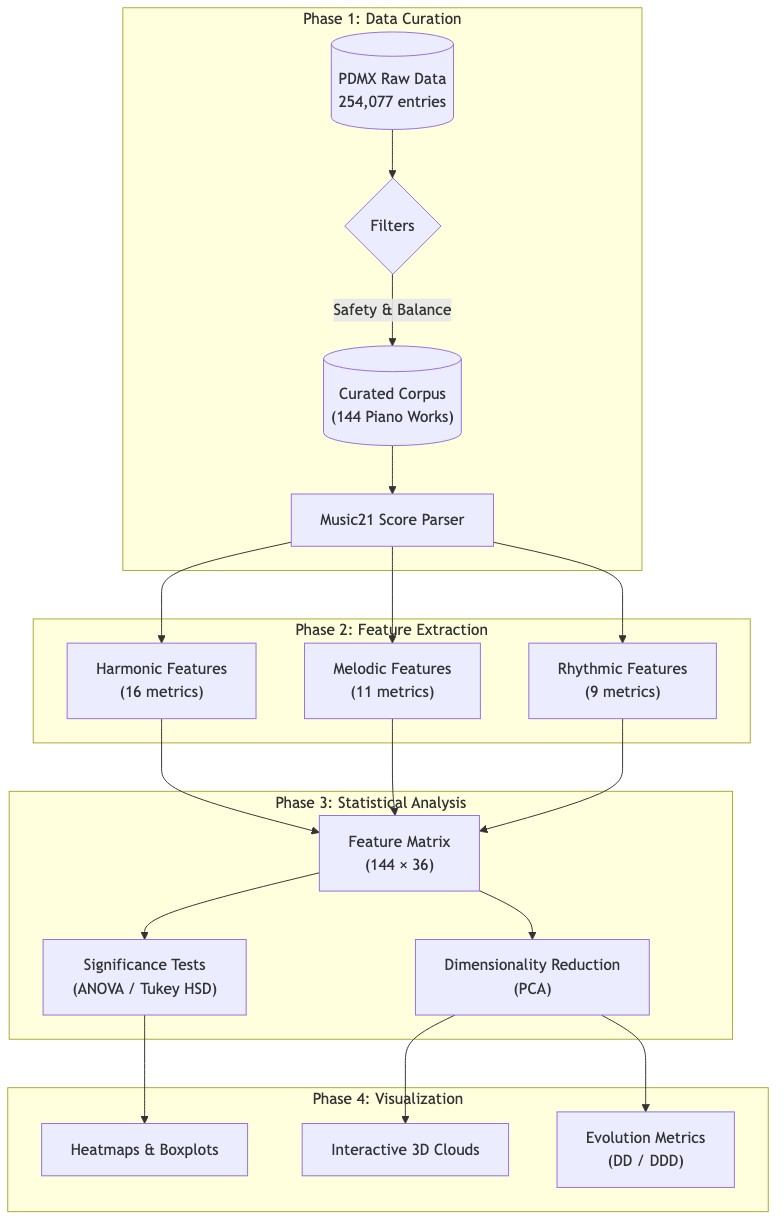
\includegraphics[width=0.85\textwidth]{figures/pipeline_architecture.png}
    \caption{Systemarchitektur der Analyse-Pipeline. Phase~1 filtert 254\,077 PDMX-Einträge auf 144 balancierte Klavierwerke. Phase~2 extrahiert 36 Merkmale in drei Kategorien. Phase~3 führt statistische Tests durch. Phase~4 erzeugt interaktive Visualisierungen und Evolutionsmetriken.}\label{fig:pipeline}
\end{figure}

\subsection{Systemvoraussetzungen und Ressourcenbedarf}

\begin{itemize}
    \item \textbf{Betriebssystem}: macOS, Linux oder Windows mit WSL
    \item \textbf{Python}: Version 3.10 oder höher
    \item \textbf{Speicherplatz}: 
    \begin{itemize}
        \item PDMX-Datensatz: $\sim$56 GB (254\,077 MusicXML-Partituren)
        \item Python Virtual Environment: $\sim$600 MB
        \item Zwischenergebnisse (Features, Statistiken, Visualisierungen): $\sim$50 MB
    \end{itemize}
    \item \textbf{Rechenzeit}: 2--3 Stunden für vollständigen Durchlauf auf modernem Laptop
    \item \textbf{RAM}: Mindestens 8 GB empfohlen (16 GB für große Bach-Choralkompilationen)
\end{itemize}

\subsection{Automatisierte Installation mit Quickstart-Skript}

Das Projekt enthält ein vollautomatisches Bash-Skript, das Installation und Analyse in einem Durchlauf erledigt.

\subsubsection{Vollautomatischer Ablauf}

\begin{lstlisting}
./quickstart.sh
\end{lstlisting}

Das Skript führt automatisch folgende Schritte aus:
\begin{enumerate}
    \item \textbf{Abhängigkeitsprüfung}: Validiert Python-Installation und \texttt{requirements.txt}
    \item \textbf{Datensatz-Download}: Bietet interaktiven Download von Zenodo (15571083) an, falls PDMX-Verzeichnis fehlt. Unterstützt \texttt{aria2c} für parallele Downloads (16 Verbindungen) mit Fallback auf \texttt{wget}
    \item \textbf{Virtual Environment}: Erstellt isolierte Python-Umgebung im \texttt{venv/}-Verzeichnis
    \item \textbf{Dependency-Installation}: Installiert \texttt{music21}, \texttt{pandas}, \texttt{numpy}, \texttt{scipy}, \texttt{scikit-learn}, \texttt{matplotlib}, \texttt{seaborn}, \texttt{plotly}
    \item \textbf{Pipeline-Ausführung}: Führt alle 10 Analyseschritte sequenziell aus (siehe unten)
\end{enumerate}

\textbf{Alternative ohne Virtual Environment:}
\begin{lstlisting}
./quickstart.sh --no-venv
\end{lstlisting}
Nutzt System-Python-Installation (für conda-Nutzer oder vorinstallierte Abhängigkeiten).

\subsection{Die 10-Stufen-Analysepipeline}

Das Quickstart-Skript orchestriert folgende Schritte:

\subsubsection{Stufe 1--2: Korpus-Kuratierung und Parsing}

\textbf{[1/10] Korpus-Kuratierung}
\begin{lstlisting}
python3 src/corpus_curation.py --min-rating 0
\end{lstlisting}
\textit{Ausgabe}: \texttt{data/curated/solo\_piano\_corpus.csv} (144~Werke), \newline\texttt{solo\_piano\_mxl\_paths.txt}

\textbf{[2/10] Struktur-Parsing}
\begin{lstlisting}
python3 src/score_parser.py \
    --output data/parsed/summaries.json
\end{lstlisting}
\textit{Ausgabe}: JSON mit Taktzahl, Stimmenzahl, Dauern pro Partitur

\subsubsection{Stufe 3--5: Merkmals-Extraktion}

\textbf{[3/10] Harmonische Merkmale}
\begin{lstlisting}
python3 src/harmonic_features.py \
    --output-csv data/features/harmonic_features.csv
\end{lstlisting}
\textit{Ausgabe}: 16 harmonische Deskriptoren + Boxplots in \texttt{figures/harmonic/}

\textbf{[4/10] Melodische Merkmale}
\begin{lstlisting}
python3 src/melodic_features.py \
    --output-csv data/features/melodic_features.csv
\end{lstlisting}
\textit{Ausgabe}: 11 melodische Deskriptoren + Boxplots in \texttt{figures/melodic/}

\textbf{[5/10] Rhythmische Merkmale}
\begin{lstlisting}
python3 src/rhythmic_features.py \
    --output-csv data/features/rhythmic_features.csv
\end{lstlisting}
\textit{Ausgabe}: 9 rhythmische Deskriptoren + Boxplots in \texttt{figures/rhythmic/}

\subsubsection{Stufe 6: Dimensionsreduktion und Embedding}

\textbf{[6/10] PCA- und t-SNE-Projektionen}
\begin{lstlisting}
# PCA mit 3D/2D-Visualisierung
python3 src/feature_embedding.py --method pca \
    --output figures/embeddings/pca_3d.html \
    --output-2d figures/embeddings/pca_2d.html \
    --loadings-csv data/stats/pca_loadings.csv \
    --clouds-output figures/embeddings/pca_clouds_3d.html \
    --clouds-output-2d figures/embeddings/pca_clouds_2d.html

# t-SNE mit angepassten Hyperparametern
python3 src/feature_embedding.py --method tsne \
    --perplexity 20 --tsne-composer-weight 4.0 \
    --output figures/embeddings/tsne_3d.html \
    --clouds-output figures/embeddings/tsne_clouds_3d.html
\end{lstlisting}
\textit{Ausgabe}: Interaktive HTML-Scatter-Plots, Gaußsche Dichtewolken, PCA-Loadings

\subsubsection{Stufe 7--8: Statistische Signifikanz}

\textbf{[7/10] ANOVA und Tukey-HSD-Tests}
\begin{lstlisting}
python3 src/significance_tests.py \
    --anova-output data/stats/anova_summary.csv \
    --tukey-output data/stats/tukey_hsd.csv
\end{lstlisting}
\textit{Ausgabe}: F-Statistiken, p-Werte, Bonferroni/FDR-Flags, paarweise Vergleiche

\textbf{[8/10] Signifikanz-Visualisierungen}
\begin{lstlisting}
python3 src/significance_visualizations.py --top-n 15
\end{lstlisting}
\textit{Ausgabe}: Bar-Charts, Heatmaps (Paar-Counts, Mean-Diff., Sym-Log) in \newline\texttt{figures/significance/}

\subsubsection{Stufe 9--10: Annotation und Aggregation}

\textbf{[9/10] Annotierte Referenzpartituren}
\begin{lstlisting}
python3 src/generate_selected_annotations.py
\end{lstlisting}
\textit{Ausgabe}: 8 farbcodierte MusicXML-Dateien (2 pro Komponist) mit Dissonanz-Labels, Akkordsymbolen und optionalen PDF-Renderings

\textbf{[10/10] Master-Aggregation}
\begin{lstlisting}
python3 src/aggregate_metrics.py
\end{lstlisting}
Validiert alle Outputs, druckt Korpus-Statistiken, verifiziert Konsistenz

\subsection{Manuelle Einzelschritte und Debugging}

\subsubsection{Schnelltests mit \texttt{--limit}}

Jedes Feature-Extraktions-Skript unterstützt partielle Läufe:
\begin{lstlisting}
python3 src/harmonic_features.py --limit 5 \
    --output-csv /tmp/harmonic_test.csv
\end{lstlisting}
Prozessiert nur die ersten 5 Partituren für Smoke-Tests.

\subsubsection{Cached Runs mit \texttt{--features-from}}

Wiederverwendung bereits berechneter Features ohne Neuberechnung:
\begin{lstlisting}
python3 src/harmonic_features.py \
    --features-from data/features/harmonic_features.csv \
    --skip-plots
\end{lstlisting}
Nutzt existierende CSV, erzeugt nur Statistiken (nützlich für iterative Visualisierungen).

\subsubsection{Alternative Korpus-Varianten}

Experimentiere mit unbalancierten oder entspannten Filtern:
\begin{lstlisting}
python3 src/corpus_curation.py --min-rating 0 \
    --skip-license-filter \
    --max-per-composer 999 \
    --output-csv data/curated/unbalanced_corpus.csv
\end{lstlisting}

\subsection{Erweiterte Funktionen}

\subsubsection{Externe Stück-Projektion}

Projiziere beliebige MusicXML-Dateien in den PCA-Raum:
\begin{lstlisting}
python3 src/highlight_pca_piece.py \
    --pieces path/to/score.mxl \
    --title "Joe Hisaishi - One Summer's Day" \
    --composer "Joe Hisaishi" \
    --output highlighted_projection.html
\end{lstlisting}
Unterstützt mehrere Stücke gleichzeitig mit individuellen Labels.

\subsubsection{MusicXML-Annotation mit MuseScore-Rendering}

Erzeuge farbcodierte Analysepartituren mit automatischem PDF-Export:
\begin{lstlisting}
python3 src/annotate_musicxml.py \
    path/to/input.mxl \
    path/to/output_annotated.mxl \
    --renderer-template "mscore -o {output} {input}" \
    --render-format pdf
\end{lstlisting}
Färbt Durchgänge (orange), Appoggiaturen (violett), andere Dissonanzen (rot), chromatische Harmonien (türkis); fügt römische Ziffern als Akkordsymbole ein.

\subsection{Validierung der Installation}

\subsubsection{Erwartete Ergebnisse}

Nach vollständigem Durchlauf sollten folgende Kennzahlen reproduziert werden:
\begin{itemize}
    \item \textbf{Korpusgröße}: Exakt 144 Partituren (36 pro Komponist)
    \item \textbf{Gesamtdauer}: 71\,585 Viertelnoten (\textasciitilde13,3 Stunden bei 90 BPM)
    \item \textbf{ANOVA-Treffer ($\alpha=0.05$)}: 29 Merkmale
    \item \textbf{FDR-robuste Merkmale ($q<0.05$)}: 29 Merkmale
    \item \textbf{PCA-Varianz (PC1--PC3)}: 48,2\% (22,3\% + 16,1\% + 9,8\%)
    \item \textbf{Tukey-Unterschiede Debussy--Mozart}: 16 signifikante Merkmale
    \item \textbf{Tukey-Unterschiede Bach--Mozart}: 10 signifikante Merkmale (bzw. 16 inklusive Zähl-/Größenmetriken)
\end{itemize}

\subsubsection{Schnelle Integritätsprüfung}

\begin{lstlisting}
# Test 1: Parsing-Integrität
python3 src/score_parser.py --limit 5 \
    --output /tmp/test_parse.json
# Erwartung: 5 erfolgreiche Parses

# Test 2: Feature-Extraktion
python3 src/harmonic_features.py --limit 5 \
    --output-csv /tmp/test_harmonic.csv
# Erwartung: 5 Zeilen mit 16 Harmonie-Spalten

# Test 3: Statistik-Pipeline
python3 src/significance_tests.py --alpha 0.05
# Erwartung: anova_summary.csv mit 36 Zeilen
\end{lstlisting}

\subsection{Häufige Probleme und Lösungen}

\begin{description}
    \item[\texttt{music21} Parse-Fehler bei manchen Partituren] Einige MusicXML-Dateien enthalten Formatfehler oder sind Opus-Kompilationen. \textbf{Lösung}: Alle Skripte verwenden standardmäßig \texttt{--skip-errors}, um fehlerhafte Dateien zu überspringen. Für Debugging: \texttt{--no-skip-errors} aktivieren.
    
    \item[Matplotlib Backend-Fehler auf Headless-Systemen] Server ohne Display benötigen nicht-interaktives Backend. \textbf{Lösung}: \texttt{export MPLBACKEND=Agg} vor Ausführung setzen.
    
    \item[Speicherprobleme bei Bach-Chorälen] Einige Bach-Werke enthalten 100+ Choräle. \textbf{Lösung}: \texttt{-{}-limit} Parameter nutzen oder RAM auf min.\ 16\,GB erhöhen.
    
    \item[Abweichende PCA-Ergebnisse trotz \texttt{random\_state=42}] Unterschiedliche \texttt{scikit-learn}-Versionen können minimal andere Rotationen erzeugen. \textbf{Lösung}: Für exakte Replikation Versionen pinnen (z.\,B. via \texttt{pip freeze > requirements-lock.txt}) und die Analyse in einer frischen Umgebung ausführen.
    
    \item[Zenodo-Download schlägt fehl] API-Rate-Limits oder Netzwerkprobleme. \textbf{Lösung}: Manueller Download von \url{https://zenodo.org/records/15571083}, Extraktion nach \texttt{15571083/}.
\end{description}

\subsection{Datenformat-Spezifikationen}

\subsubsection{Korpus-CSV (\texttt{data/curated/solo\_piano\_corpus.csv})}
\begin{itemize}
    \item \texttt{composer\_label}: Normalisiert (Bach | Mozart | Chopin | Debussy)
    \item \texttt{title}: Werktitel aus PDMX-Metadaten
    \item \texttt{mxl}: Relativer Pfad zu MusicXML-Datei (z.\,B.\ \texttt{0/46/Qmaug5p...mxl})
    \item \texttt{rating}: PDMX-Qualitätsbewertung (0.0--5.0)
    \item \texttt{subset:*}: Boolsche Flags für PDMX-Subsets
\end{itemize}

\subsubsection{Feature-CSVs (\texttt{data/features/*.csv})}
Einheitliches Format für alle drei Feature-Typen:
\begin{itemize}
    \item \texttt{composer}: Komponistenname (für Gruppierung in ANOVA)
    \item \texttt{title}: Werktitel
    \item Feature-Spalten: Numerische Werte (NaN bei Extraktionsfehlern)
\end{itemize}

\subsubsection{ANOVA-Ergebnisse (\texttt{data/stats/anova\_summary.csv})}
\begin{itemize}
    \item \texttt{feature}: Merkmalsname
    \item \texttt{F\_statistic}: ANOVA-F-Wert
    \item \texttt{p\_value}: Nicht-adjustierter p-Wert
    \item \texttt{bonferroni\_sig}: Bonferroni-Signifikanz (nach $\alpha/36$)
    \item \texttt{fdr\_sig}: Benjamini-Hochberg FDR-Signifikanz ($q<0.05$)
\end{itemize}

\subsubsection{Tukey-Ergebnisse (\texttt{data/stats/tukey\_hsd.csv})}
\begin{itemize}
    \item \texttt{feature}: Merkmalsname
    \item \texttt{group1}, \texttt{group2}: Komponistenpaar
    \item \texttt{meandiff}: Mittlere Differenz
    \item \texttt{lower}, \texttt{upper}: 95\%-Konfidenzintervall
    \item \texttt{reject}: Signifikanz (True/False)
\end{itemize}

\clearpage
\section{Online-Links und Indexseiten}\label{app:C}


Alle Abbildungen im PDF sind klickbar und führen zu den interaktiven Online-Versionen. Zur Sicherheit sind alle Links hier gesammelt aufgeführt (für Leserinnen und Leser ohne PDF-Link-Unterstützung).

\subsection{Index-Startseiten}
\begin{itemize}
    \item \textbf{Gesamtindex der Abbildungen}: \newline\linkurl{https://victor-gurbani.github.io/JuFo2026/figures/}
    \item \textbf{Embeddings (PCA/t-SNE)}: \newline\linkurl{https://victor-gurbani.github.io/JuFo2026/figures/embeddings/}
    \item \textbf{Highlights (externe Stücke)}: \newline\linkurl{https://victor-gurbani.github.io/JuFo2026/figures/highlights/}
    \item \textbf{Signifikanz-Plots}: \newline\linkurl{https://victor-gurbani.github.io/JuFo2026/figures/significance/}
    \item \textbf{Harmonische Boxplots}: \newline\linkurl{https://victor-gurbani.github.io/JuFo2026/figures/harmonic/}
    \item \textbf{Melodische Boxplots}: \newline\linkurl{https://victor-gurbani.github.io/JuFo2026/figures/melodic/}
    \item \textbf{Rhythmische Boxplots}: \newline\linkurl{https://victor-gurbani.github.io/JuFo2026/figures/rhythmic/}
    \item \textbf{Annotierte MusicXML-Dateien}: \newline\linkurl{https://victor-gurbani.github.io/JuFo2026/figures/annotated/}
\end{itemize}

\subsection{Direktlinks zu interaktiven Kernansichten}
\begin{itemize}
    \item \textbf{PCA-Komponistenwolken (3D)}: \newline\linkurl{https://victor-gurbani.github.io/JuFo2026/figures/embeddings/composer_clouds_3d.html}
    \item \textbf{Highlight: One Summer's Day (Hisaishi)}: \newline\linkurl{https://victor-gurbani.github.io/JuFo2026/figures/highlights/one_summers_day_pca_cloud.html}
    \item \textbf{Highlight: Ravel String Quartet (F-Dur)}: \newline\linkurl{https://victor-gurbani.github.io/JuFo2026/figures/highlights/ravel_string_quartet_pca_cloud.html}
\end{itemize}

\subsection{Software-Lizenzierung und Zitierung}

\begin{itemize}
    \item \textbf{PDMX-Datensatz}: Public Domain, verfügbar unter \url{https://zenodo.org/records/15571083}. Zitierung: \cite{PDMX2024}
    \item \textbf{Repository}: \href{https://github.com/victor-gurbani/JuFo2026/}{\faGithub\ github.com/victor-gurbani/JuFo2026}
    \item \textbf{Analysecode}: Siehe \texttt{LICENSE}-Datei im Repository
    \item \textbf{Extrahierte Features}: Abgeleitete Daten, frei verwendbar für akademische Zwecke unter Nennung dieser Arbeit
    \item \textbf{Dependencies}: Alle verwendeten Bibliotheken (\texttt{music21}, \texttt{scikit-learn}, etc.) sind Open Source (BSD/MIT-Lizenzen)
\end{itemize}

Dieser Leitfaden ermöglicht vollständige Reproduktion aller Ergebnisse sowie deren Erweiterung auf neue Fragestellungen. Bei Problemen: GitHub-Issues im Repository oder Kontakt über verfügbare Adresse.

\clearpage
\section{Erweiterte Details zur Machine-Learning-Pipeline}\label{app:D}

Um die Transparenz und Reproduzierbarkeit der durchgeführten Klassifikationsexperimente (Random Forest und Neuronales Netz) weiter zu erhöhen, werden in diesem Anhang tiefere Einblicke in die Hyperparameter-Optimierung, die Baumstrukturen und die lokalen SHAP-Erklärungen gegeben.

\subsection{Vergleich mit neuronalen Netzen (MLP)}
Parallel zum Random Forest wurde ein \textit{Multi-Layer Perceptron} (MLP) trainiert. Dieses neuronale Netz durfte den vollen Merkmalsraum (30 Features) ohne Vorfilterung oder Komplexitätsbeschränkung nutzen. Es diente als Referenz für das theoretisch erreichbare Maximum an Genauigkeit auf dem 144-Stücke-Datensatz.

Das Ergebnis war überraschend: Der interpretierbare RF schnitt mit $70{,}1\,\%$ Genauigkeit leicht besser ab als das unbeschränkte neuronale Netz ($68{,}7\,\%$; vgl. \hyperref[fig:nn_comparison]{Abbildung~\ref*{fig:nn_comparison}}). Wir interpretieren diesen Befund dahingehend, dass die Kombination aus Kollinearitätsfilterung und striktem Pruning als effektive Regularisierung wirkte. Während das neuronale Netz auf dem relativ kleinen Datensatz (144 Werke) zu leichtem Overfitting neigte, zwang die interpretierbare Architektur das Modell dazu, sich auf die robustesten musikalischen Merkmale -- wie den Tonumfang und die harmonische Dichte -- zu konzentrieren (\hyperref[fig:rf_scatter]{Abbildung~\ref*{fig:rf_scatter}}).

\begin{figure}[htbp]
    \centering
    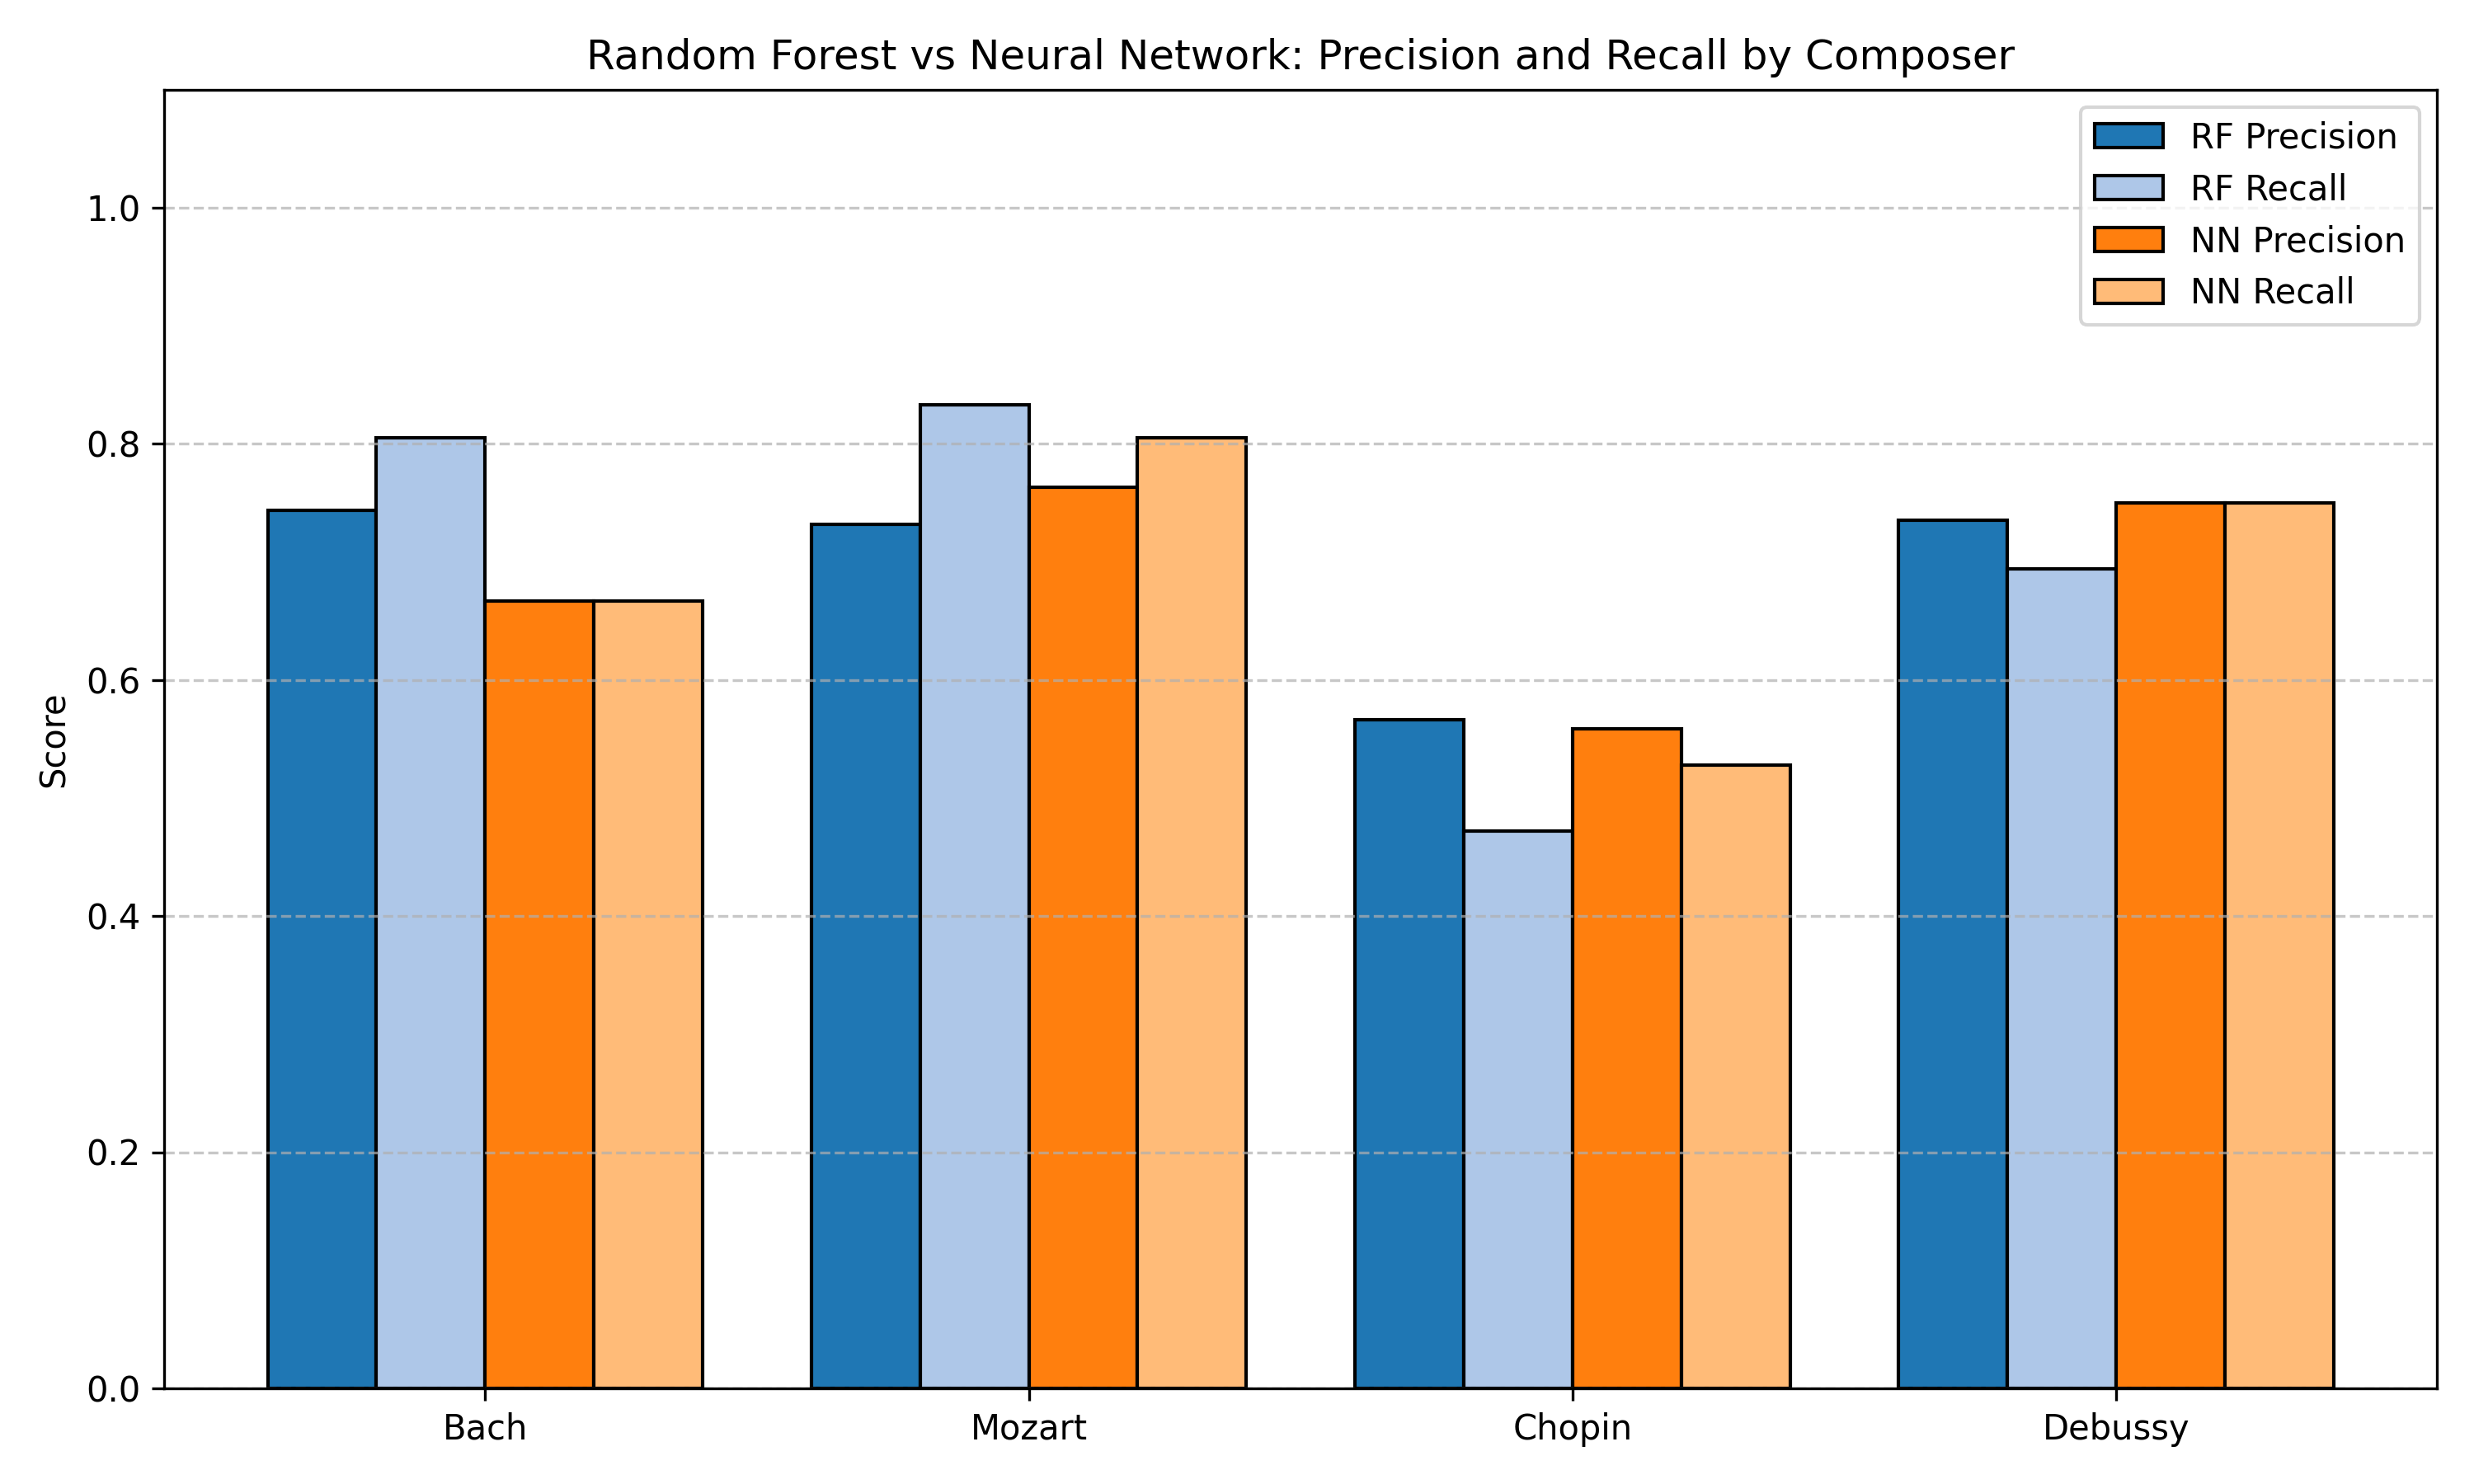
\includegraphics[width=0.75\textwidth]{figures/random_forest/nn_vs_rf_comparison.png}
    \caption{Vergleich der Klassifikationsleistung: Der interpretierbare Random Forest (RF) erzielt trotz seiner Komplexitätsbeschränkung eine leicht höhere Genauigkeit als das neuronale Netz (MLP). Die Filterung redundanter Merkmale fungiert hier als effiziente Regularisierung.}\label{fig:nn_comparison}
\end{figure}

\subsection{Hyperparameter-Optimierung und Pruning-Statistiken}
Das Training des interpretierbaren Random Forests zielte auf eine maximale Reduktion der Komplexität ab, um \enquote{White-Box}-Eigenschaften zu bewahren, ohne die Genauigkeit drastisch zu opfern. Die Optimierung erfolgte mittels \texttt{RandomizedSearchCV} (5-Fold Cross-Validation) über folgendes Raster:
\begin{itemize}
    \item \texttt{n\_estimators}: [100, 200, 300]
    \item \texttt{max\_depth}: [5, 10, 15, 20]
    \item \texttt{min\_samples\_leaf}: [2, 3, 4]
    \item \texttt{ccp\_alpha}: [0.005, 0.01, 0.015, 0.02, 0.03]
\end{itemize}

Um den konkreten Effekt des \textit{Cost-Complexity Prunings} (\texttt{ccp\_alpha}) zu quantifizieren, wurde ein komplett unbeschränkter Basis-Forest mit dem optimierten, beschnittenen Forest verglichen.
\begin{itemize}
    \item \textbf{Unpruned Baseline}: 73,61\,\% Genauigkeit, $\varnothing$ Baumtiefe: 7,90, Gesamtzahl der Knoten: 5.094
    \item \textbf{Best Pruned Model} (\texttt{ccp\_alpha=0.01}): 70,14\,\% Genauigkeit, $\varnothing$ Baumtiefe: 6,66, Gesamtzahl der Knoten: 3.270
\end{itemize}
Der Verzicht auf nur $\sim$3,5\,\% Genauigkeit führte zu einer massiven Reduzierung der Modellkomplexität um \textbf{35,8\,\% weniger Entscheidungsknoten}.

\subsection{Beispielhafter Entscheidungsbaum}
Ein Random Forest trifft Vorhersagen durch einen Mehrheitsentscheid vieler individueller Bäume. Um die Nachvollziehbarkeit zu demonstrieren, wurde der mathematisch akkurateste Einzelbaum aus dem 100-Bäume-Ensemble (Baum \#71) extrahiert. Dieser Baum erreichte alleingestellt eine Genauigkeit von 72,4\,\% auf dem Testset. Zur Gewährleistung uneingeschränkter Transparenz (\enquote{White-Box}-Paradigma) exportiert die Pipeline zudem alle 100 Entscheidungsbäume vollständig als grafische und textuelle Regelwerke zur manuellen Auditierung.

\begin{figure}[htbp]
    \centering
    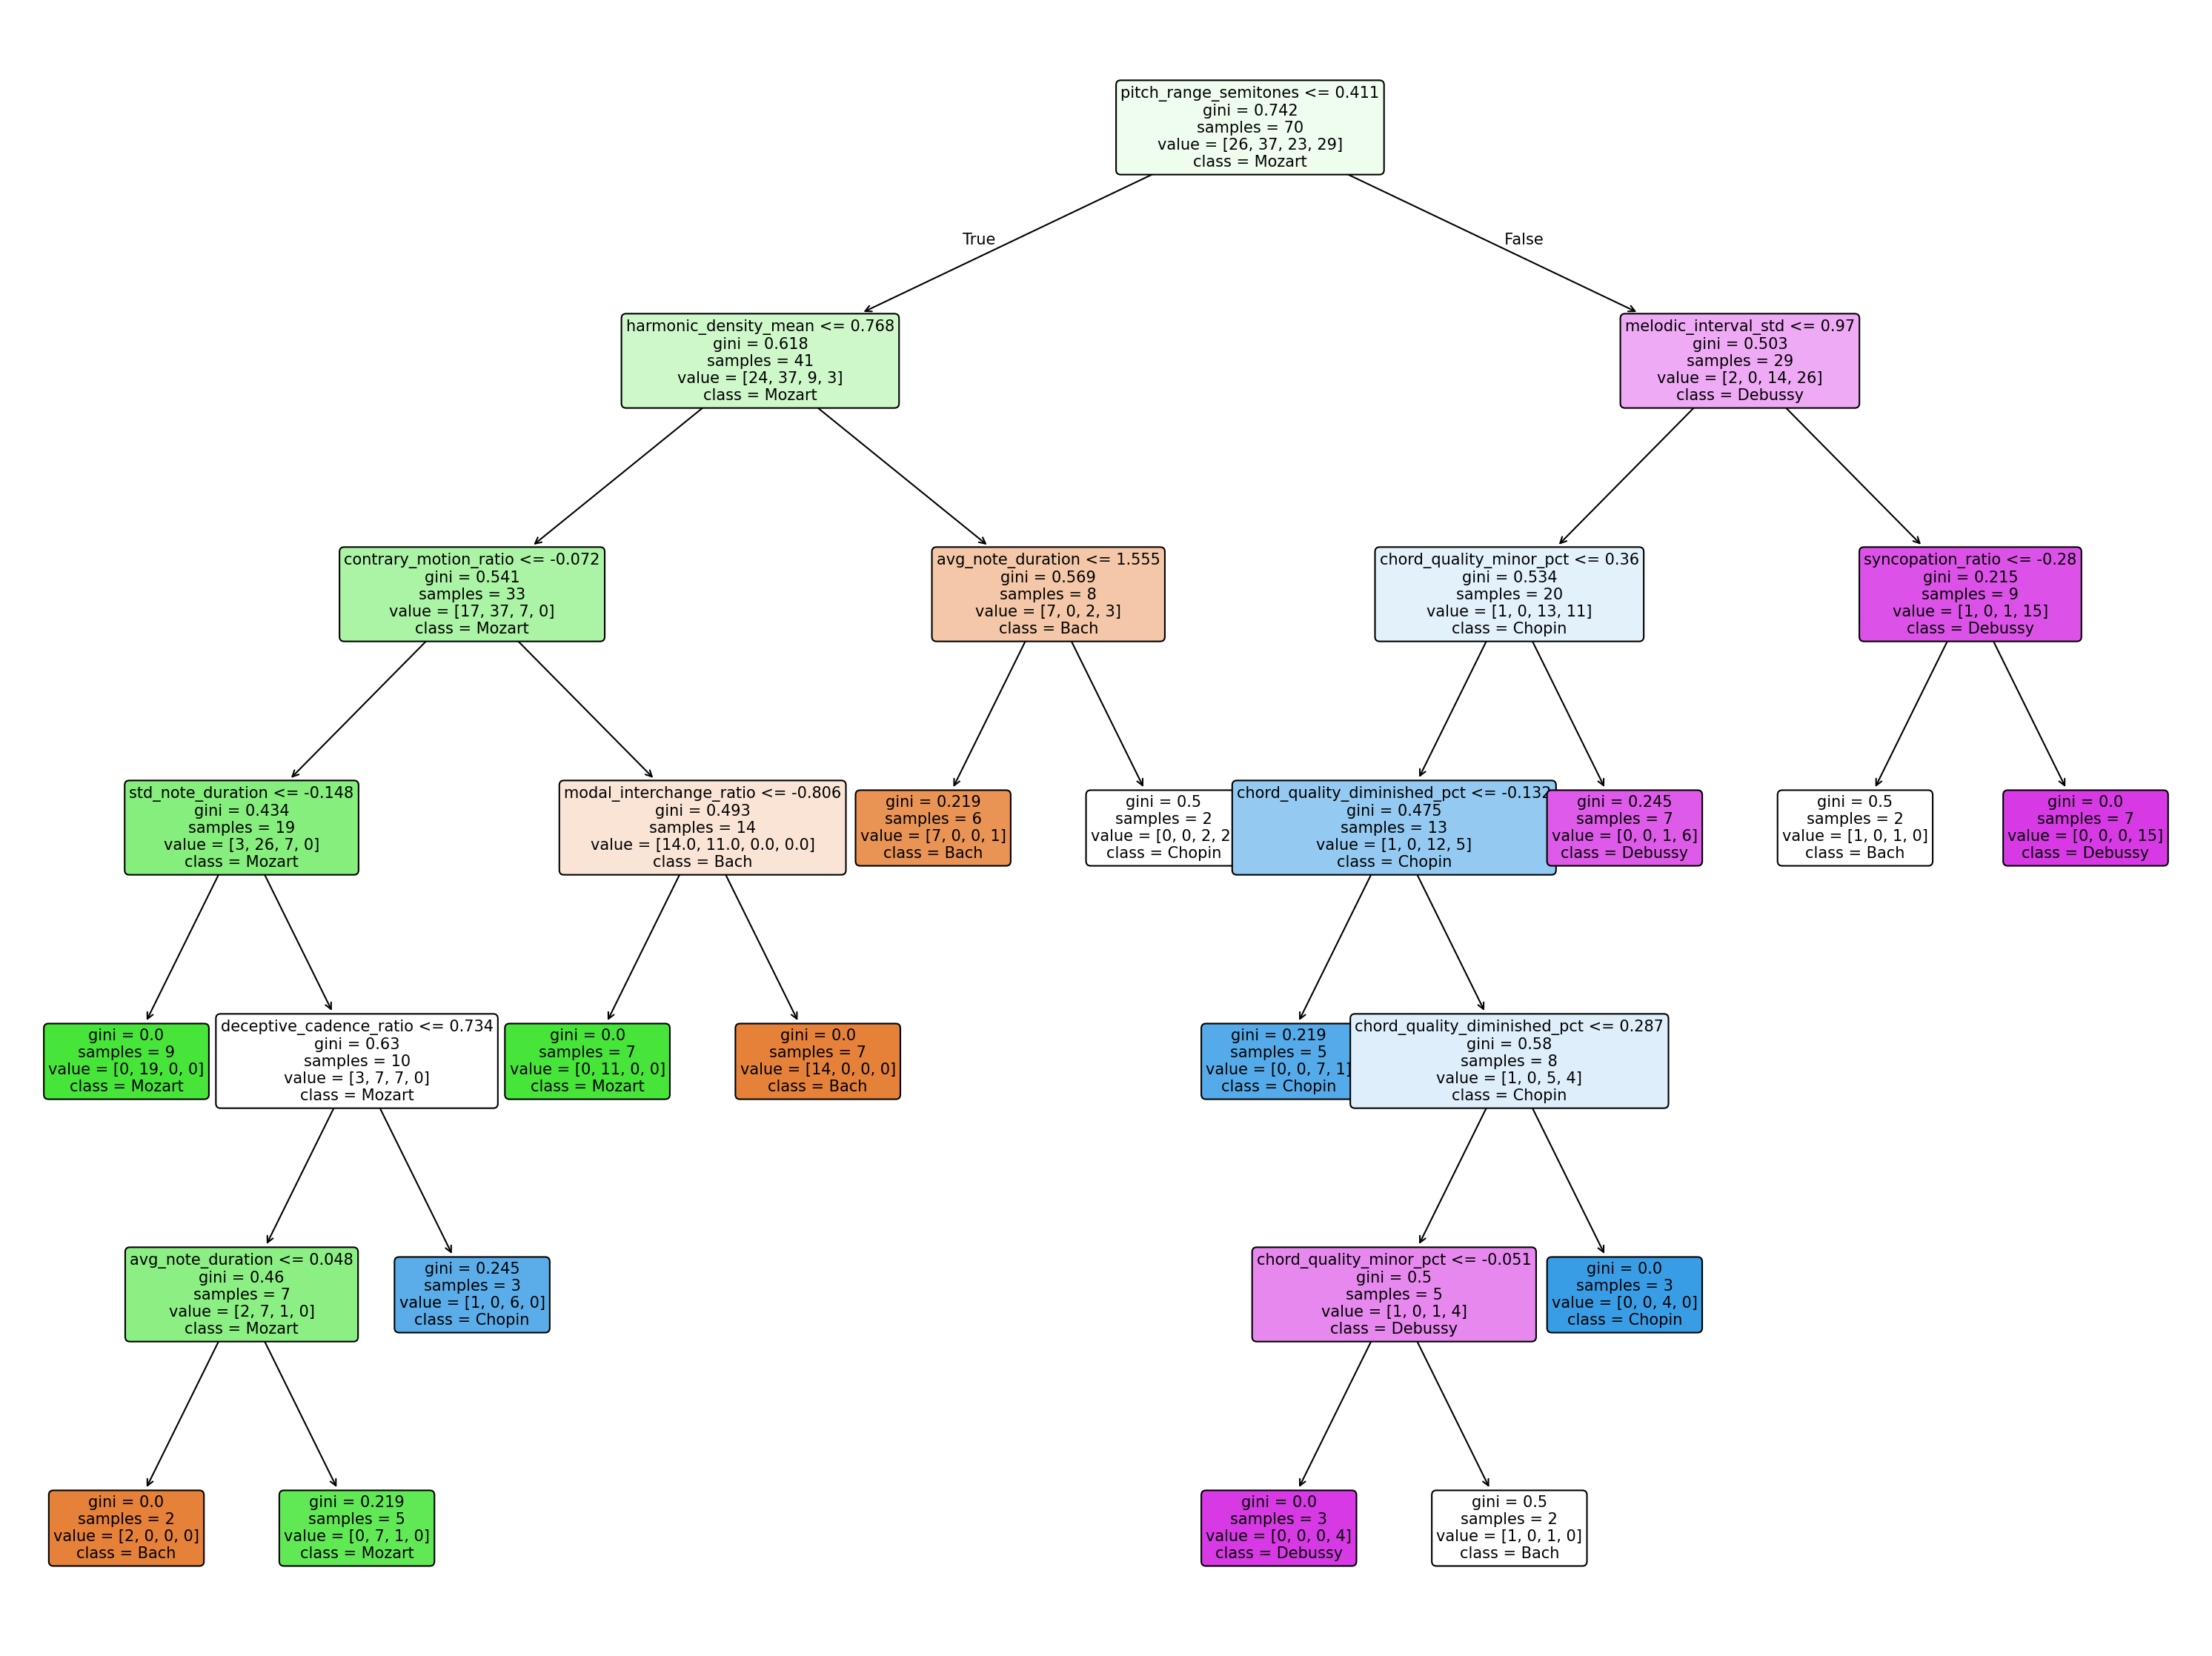
\includegraphics[width=\textwidth]{figures/random_forest/rf_sample_tree.png}
    \caption{Der akkurateste Einzelbaum des Random-Forest-Ensembles. Jeder Knoten zeigt das Entscheidungskriterium (Merkmal), die Gini-Impurity (Grad der Mischung), die verbleibende Anzahl von Stücken (Samples) und deren Verteilung auf die vier chronologischen Klassen: [Bach, Mozart, Chopin, Debussy].}\label{fig:rf_tree}
\end{figure}

\subsection{Komponistenspezifische SHAP-Analysen}
Während einzelne Entscheidungsbäume eine \textit{Mikro-Logik} zeigen, aggregieren SHAP-Werte (SHapley Additive exPlanations) die spieltheoretischen Einflüsse aller Merkmale über das \textit{gesamte} Ensemble. Da die Merkmale im Vorfeld mittels Spearman-Clustering von Kollinearität befreit wurden, zeigen diese Plots die isoliertesten und aussagekräftigsten Unterscheidungsmerkmale. Dass diese sich teilweise von den Top-Merkmalen der ANOVA/PCA unterscheiden, liegt methodisch in der Natur des Modells: Während die statistischen Tests lineare, isolierte Varianzen messen, erfasst der Random Forest \textit{nicht-lineare, konditionale Interaktionen} (z.\,B. \enquote{Wenn Merkmal X niedrig ist, trennt Merkmal Y perfekt}) und optimiert ausschließlich auf die Klassifikationsgrenze statt auf die globale Datenvarianz.

\begin{figure}[htbp]
    \centering
    \begin{minipage}{0.48\textwidth}
        \centering
        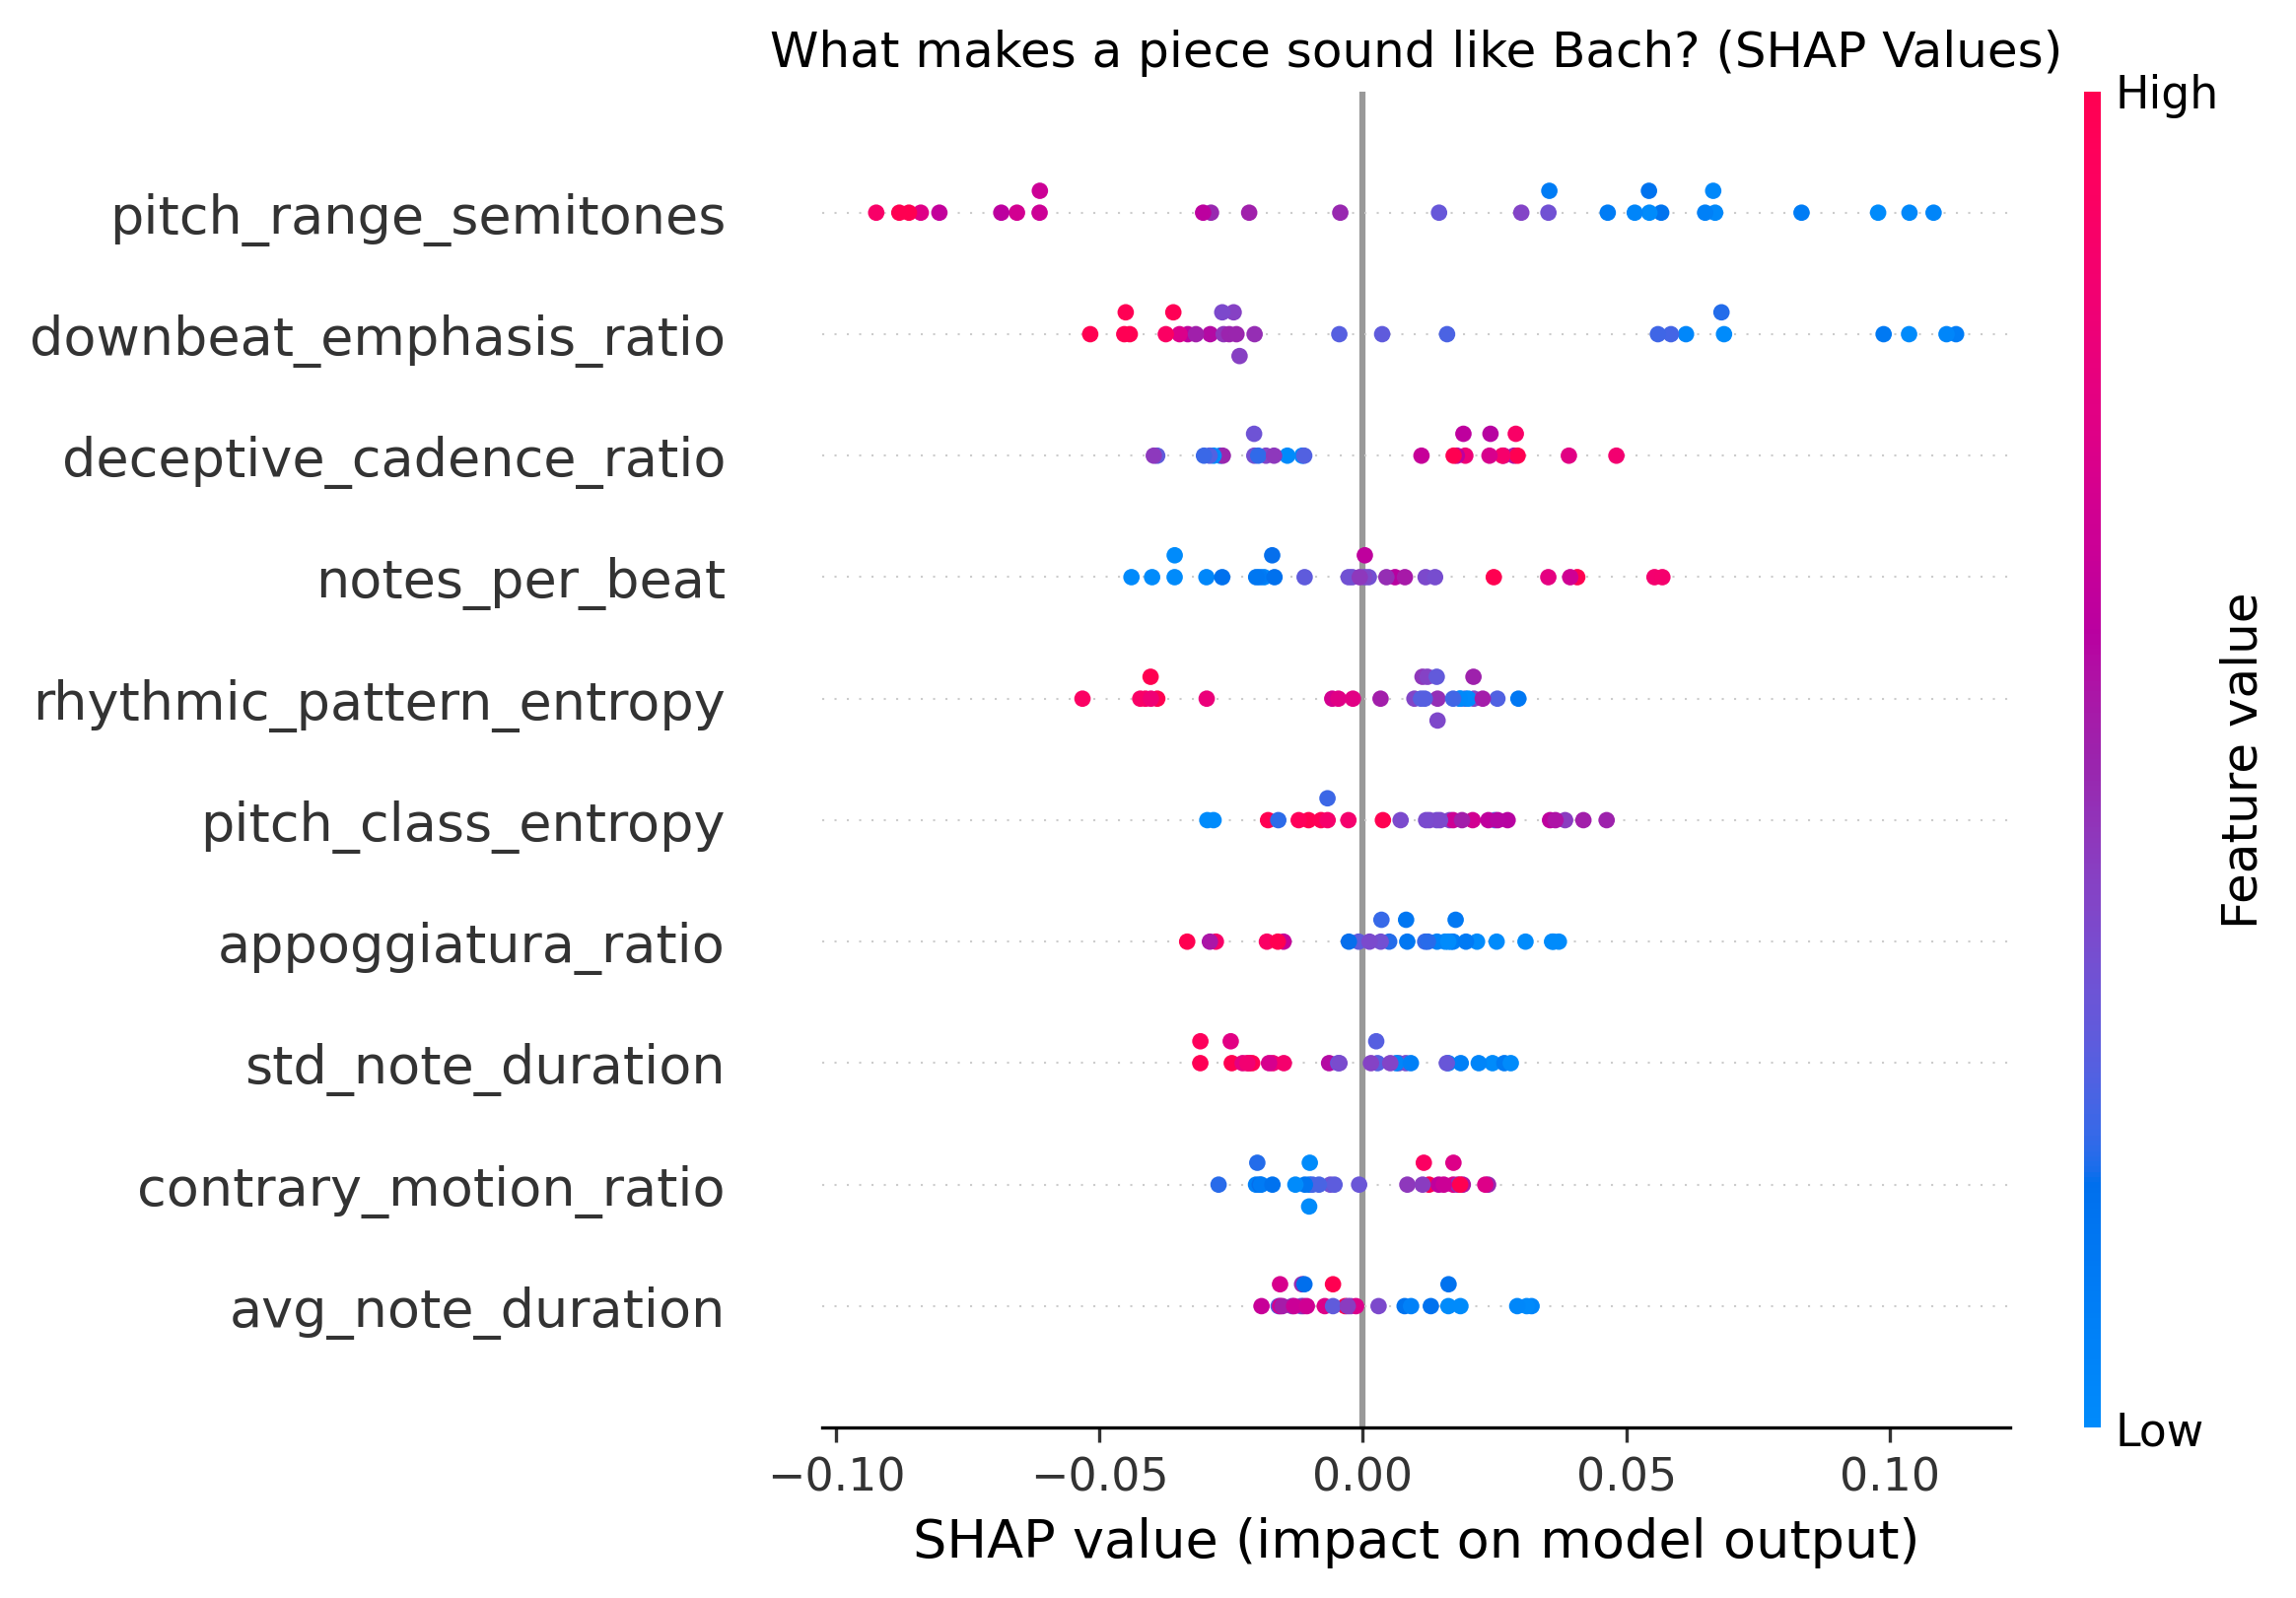
\includegraphics[width=\textwidth]{figures/random_forest/rf_shap_summary_Bach.png}
        \caption{SHAP-Werte für Johann Sebastian Bach. Niedrige Werte (blau) beim Tonumfang (\texttt{pitch\_range\_semitones}) und der Downbeat-Betonung (\texttt{downbeat\_emphasis\_ratio}) führen zu positiven SHAP-Werten (rechts der vertikalen Linie) und erhöhen somit die Wahrscheinlichkeit für Bach. Im Gegensatz dazu deuten hohe Werte (rot) bei Trugschlüssen (\texttt{deceptive\_cadence\_ratio}) und den Noten pro Taktschlag (\texttt{notes\_per\_beat}) stark auf Bach hin.}
    \end{minipage}\hfill
    \begin{minipage}{0.48\textwidth}
        \centering
        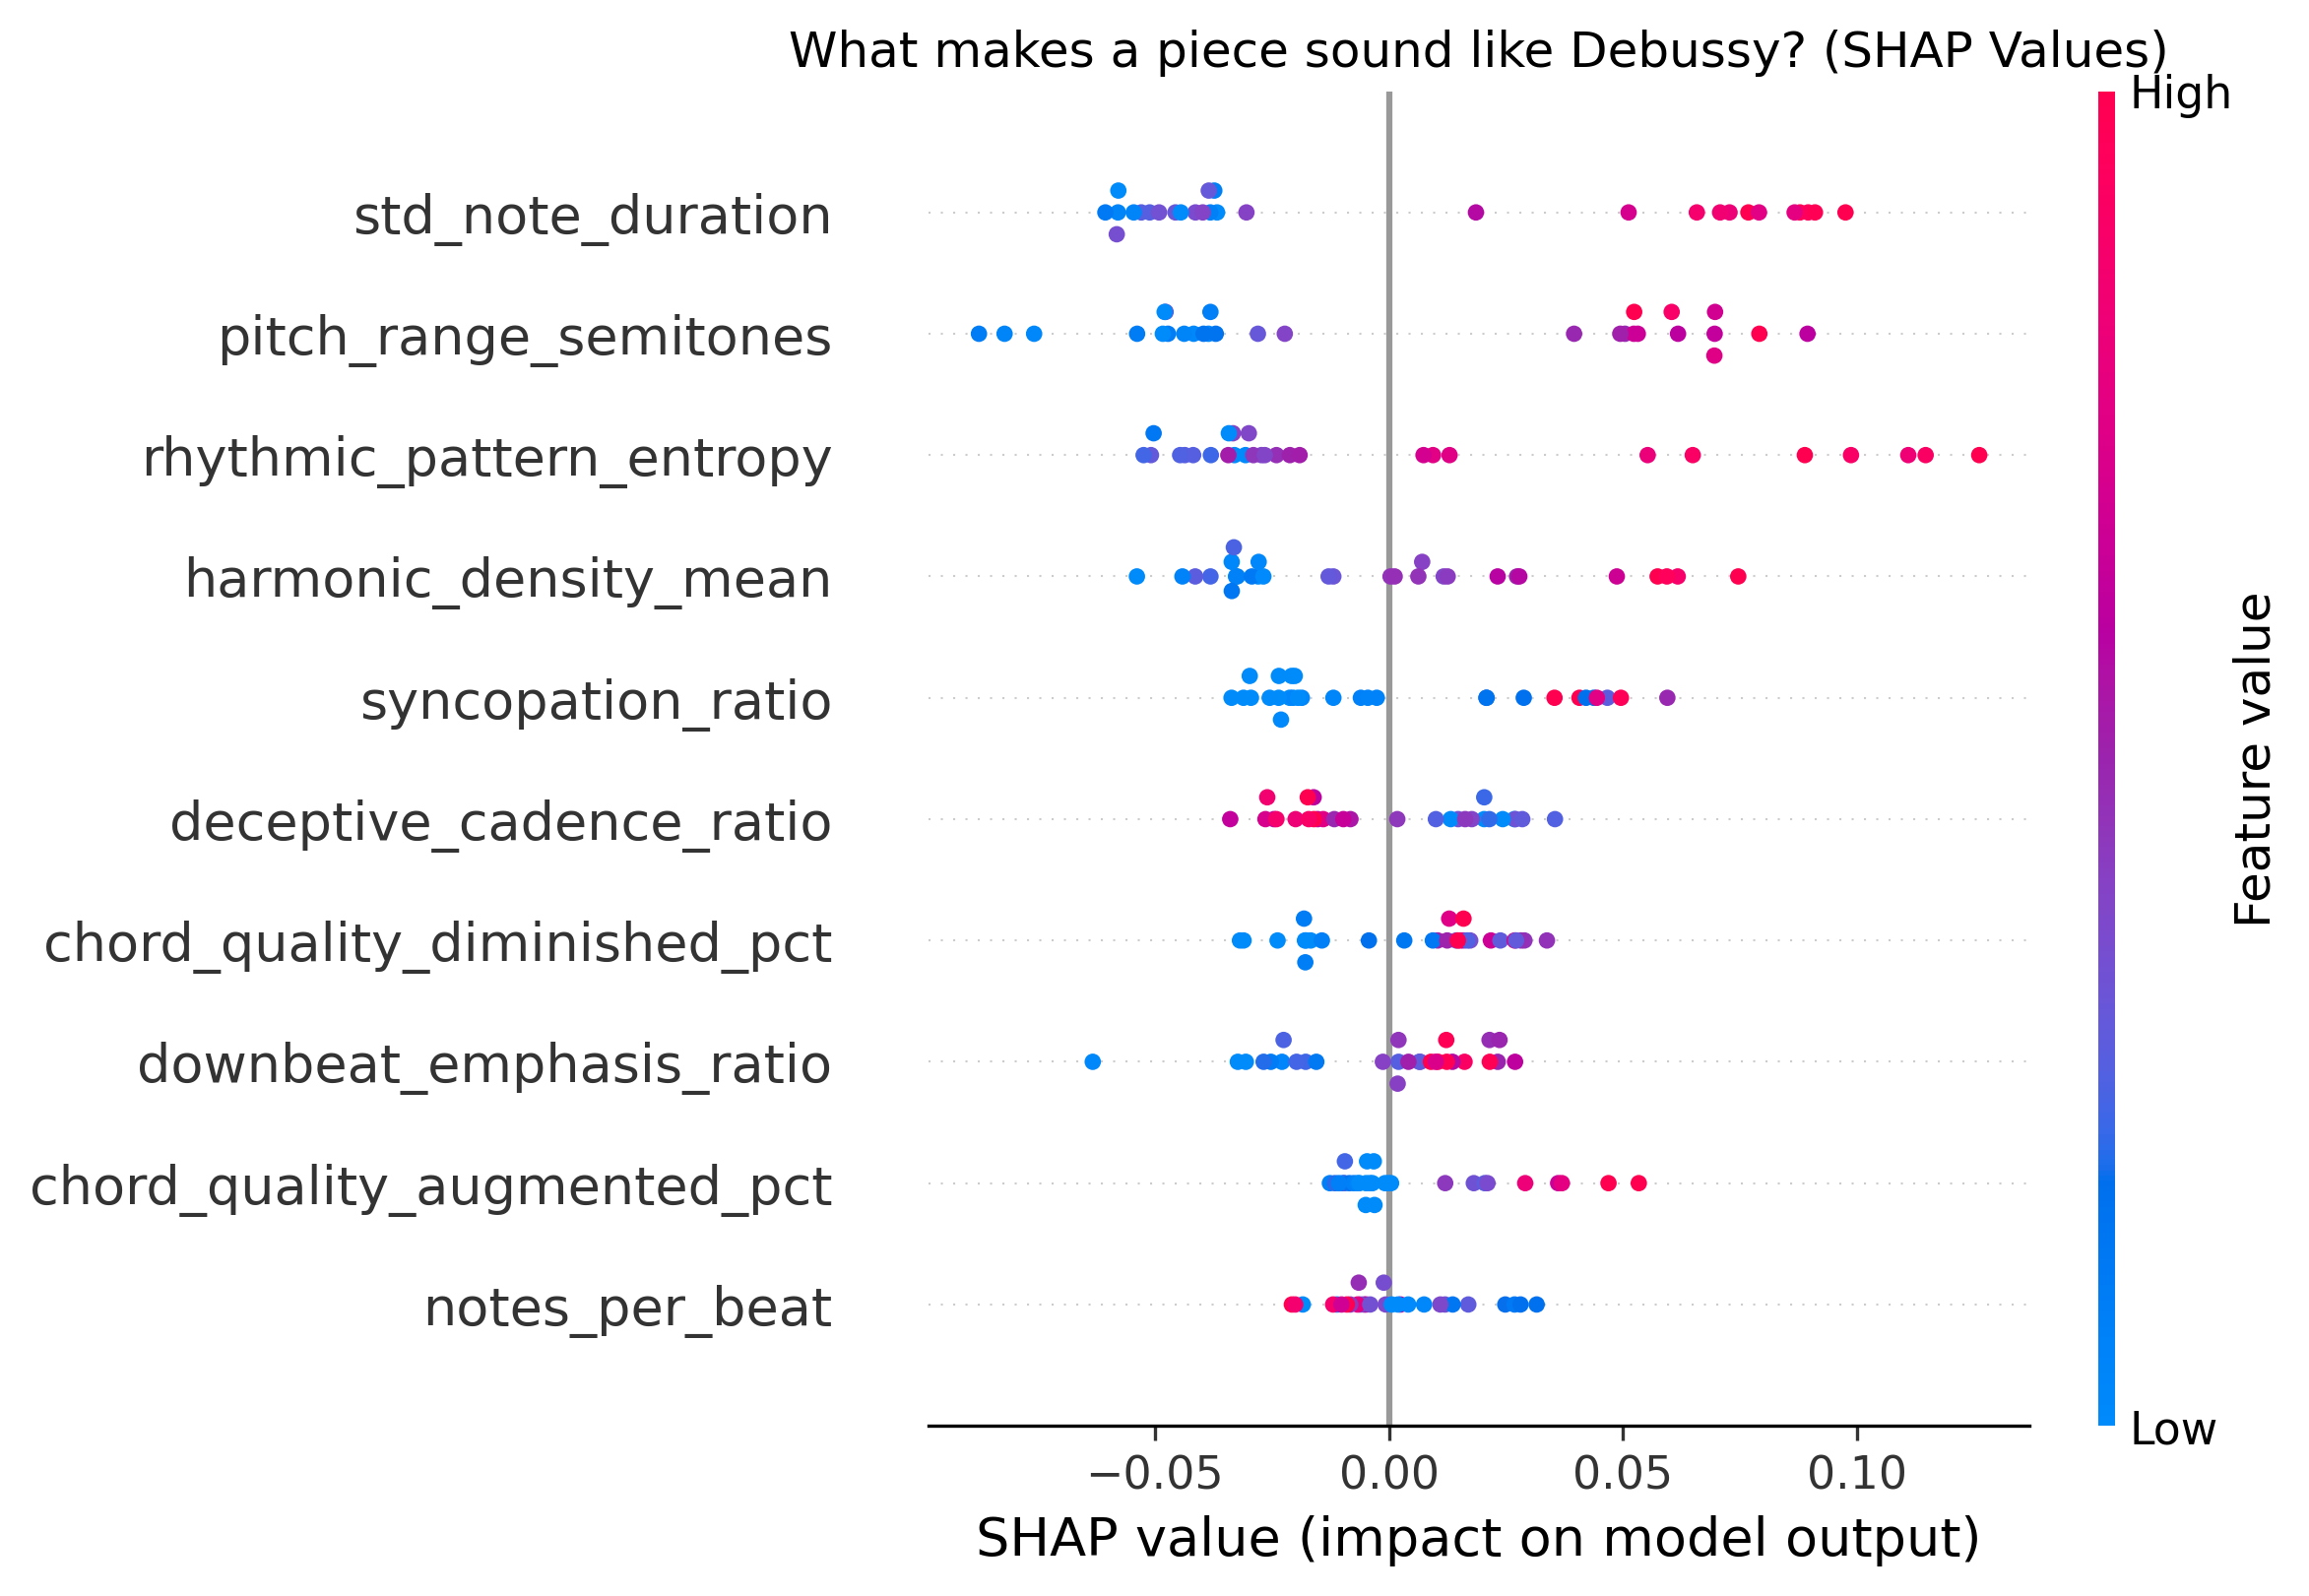
\includegraphics[width=\textwidth]{figures/random_forest/rf_shap_summary_Debussy.png}
        \caption{SHAP-Werte für Claude Debussy. Hohe Werte (rot) bei der rhythmischen Varianz (\texttt{std\_note\_duration}), dem Tonumfang (\texttt{pitch\_range\_semitones}), der rhythmischen Entropie (\texttt{rhythmic\_pattern\_entropy}) und der harmonischen Dichte (\texttt{harmonic\_density\_mean}) erzeugen positive SHAP-Werte (rechts der vertikalen Linie) und sind starke Indikatoren für Debussy. Umgekehrt sprechen niedrige Werte (blau) bei der Trugschlussrate (\texttt{deceptive\_cadence\_ratio}) eher für Debussy.}
    \end{minipage}
\end{figure}

\clearpage
\section{Deployment und Web-Infrastruktur}\label{app:E}

Die Überführung der lokalen Next.js-Datenvisualisierung in eine öffentliche Web-Anwendung erforderte die Überwindung spezifischer infrastruktureller und softwarearchitektonischer Hürden. Die Applikation (gehostet auf \linkurl{https://empirical-music.victorgurbani.com}) läuft auf einem ressourcenlimitierten Oracle Linux Virtual Private Server (VPS) unter Apache 2.4 und PM2. Die Beschränkungen in Speicher und Arbeitsspeicher setzten signifikante Optimierungen des Build-Prozesses voraus.

\subsection{Limitierungen der Standalone-Kompilierung}
Typischerweise verarbeitet das Next.js-Build-System (\texttt{Turbopack}) serverseitige Abhängigkeiten, indem es die im Quellcode verknüpften Ordnerstrukturen analysiert und in die endgültige Build-Datei integriert. In diesem Projekt operiert das Dashboard jedoch eng verzahnt mit dem Python-Backend und seinen Datensätzen (über 40\,GB an MusicXML-Dateien, extrahierten Features und gepickelten Modellen). Da Turbopack Aufrufe wie \texttt{path.join(repoRoot, rawPath)} für die serverseitigen API-Routen erfasste, versuchte der Compiler, diese gesamten 40\,GB als potenziell erforderliche serverseitige Fallback-Assets in den lokalen Build-Ordner (\texttt{.next/standalone}) zu kopieren. Dies stürzte in Schleifen ab (ENOSPC: No space left on device) oder überlastete den Arbeitsspeicher massiv.

Die Lösung war die Implementierung untrackbarer String-Interpolations-Polymorphismen in Next.js: Anstelle direkter standardisierter Bibliotheksaufrufe wertet das System die Suchpfade nun dynamisch über Laufzeit-Strings (\texttt{const joinPath = (base, ...parts) => [base, ...parts].join(path.sep)}) aus. Dadurch kompilierte Next.js in einen schmalen 50\,MB-Microserver, ohne die Datensatz-Binärdateien einzubetten. 

\subsection{Abruf dynamischer Cloud-Jobs}
Weitere Hürden betrafen die dynamische Darstellung frisch berechneter PCA-Wolken. Im \texttt{standalone}-Modus \enquote{friert} der interne Node.js-Server von Next.js seinen statischen Datei-Router (für Assets innerhalb von \texttt{/public}) zum Zeitpunkt der Kompilierung ein. Starten Besucher der Webseite jedoch im Hintergrund einen Python-Subprozess, um eine neue Datensatzwolke zu berechnen, wurden die frisch generierten Metadaten (\texttt{.json} und \texttt{.html}) unter \texttt{public/generated/clouds/} vom Standalone-Server als 404 (Not Found) blockiert. Um dies zu umgehen, wurde in der Apache-Konfiguration ein Reverse-Proxy-Bypass integriert. Apache fängt Anfragen, die sich an die Verzeichnisse \texttt{/img} oder \texttt{/generated} richten (\texttt{Alias /generated /var/www/jufo2026/web-interface/public/generated}), explizit ab und serviert die frisch verfassten Dokumente nativ aus dem VPS-Dateisystem, während alle React- und API-spezifischen Endpunkte an den PM2-gewrappten Next.js-Dienst auf Port 3011 weitergeleitet werden. 

\subsection{Das Caching-Resolver-Dilemma}\label{sec:caching}
Schlussendlich trat das Problem der Interoperabilität von Dateipfaden zwischen macOS-Entwicklungssystemen und Oracle-Linux-Hosting auf. Das Backend speicherte Caches mit absoluten Unix-Dateipfaden der MusicXML-Dateien, um Dimensionsreduktions-Metadaten effizienter heranzuziehen. Da die korrespondierenden MusicXML-Dateien aus Speicher-Gründen nicht auf den Server mitkopiert wurden (\texttt{--forceCache}-Flag überschreibt den Verzeichnis-Check), litten die Identifizierungs-Signaturen im Skript \texttt{embedding\_cache.py} unter fehlschlagenden Zuordnungen. Durch den Umbau der Abgleichoperation mithilfe von \texttt{Path(mxl\_abs\_path).name.endswith(...)} wurde gewährleistet, dass das Dashboard auch dann voll funktionsfähig agiert und Einzelstücke fehlerfrei visualisiert rekonstruieren kann, wenn nur der Feature-Cache der Pipeline lokalisiert wird, selbst in Cross-OS-Szenarien ohne korrespondierenden Rohdatensatz.


\section{Multicore-Caching-Infrastruktur}\label{app:F}
Um Analysen auf das vollständige PDMX-Archiv (254\,077 Partituren) zu ermöglichen, wurde ein skalierbares Caching-System entwickelt (\texttt{src/embedding\_cache.py}). Dieses System unterstützt:
\begin{itemize}
    \item \textbf{Parallelisierte Feature-Extraktion}: Die Option \texttt{--workers N} verteilt die Berechnung auf $N$ CPU-Kerne. Bei 8 Kernen beschleunigt sich die Verarbeitung um den Faktor $\approx$6--7 (limitiert durch I/O).
    \item \textbf{Unterbrechungsresistenz}: Der Fortschritt wird zeilenweise in die Cache-CSV geschrieben und in einer Sidecar-Datei (\texttt{*.done.txt}) protokolliert. Mit \texttt{--resume} kann eine unterbrochene Berechnung jederzeit fortgesetzt werden -- ideal für tagelange Läufe auf großen Korpora.
    \item \textbf{Vollständiger Feature-Cache}: Neben den 3D-PCA-Koordinaten speichert das System optional alle 36 Feature-Werte pro Partitur (\texttt{--output-features-csv}). Dies ermöglicht \textit{instant subset-specific PCA}: Für beliebige Komponisten-Kombinationen kann die PCA ohne erneutes Parsen der MusicXML-Dateien sofort neu berechnet werden.
\end{itemize}

\noindent Die Cache-Integrität wird durch SHA256-Hashes der Eingabe-Feature-CSVs und JSON-Metadaten gewährleistet. Ein vollständiger Cache des PDMX-Korpus (alle 254\,077 Partituren $\times$ 36 Features) belegt etwa 180\,MB und ermöglicht Echtzeit-Exploration beliebiger Komponisten-Subsets über die Weboberfläche (siehe \hyperref[sec:weboberflache]{Abschnitt~\ref*{sec:weboberflache}}).

\end{document}
